\documentclass{article}

\usepackage{arxiv}

\usepackage[utf8]{inputenc} % allow utf-8 input
\usepackage[T1]{fontenc}    % use 8-bit T1 fonts
\usepackage{hyperref}       % hyperlinks
\usepackage{url}            % simple URL typesetting
\usepackage{booktabs}       % professional-quality tables
\usepackage{amsfonts}       % blackboard math symbols
\usepackage{nicefrac}       % compact symbols for 1/2, etc.
\usepackage{microtype}      % microtypography
\usepackage{lipsum}
\usepackage{upgreek}
\usepackage{graphicx}
\usepackage{setspace}
\usepackage{tgtermes}
\usepackage{subfig}
\usepackage[version=4]{mhchem}
\usepackage{threeparttable}
\onehalfspacing
\graphicspath{figures/}
\usepackage{array, booktabs}
\setlength{\arrayrulewidth}{0.5mm}
\setlength{\tabcolsep}{8pt}
\renewcommand{\arraystretch}{1.5}
\title{Carbon cathodes for rechargeable aluminium-ion batteries}
\author{
  Shalini Divya\\
  School of Chemical and Physial Sciences\\
  Victoria University of Wellington\\
  Wellington, New Zealand\\
  \texttt{shalini.divya@vuw.ac.nz}\\
  %% examples of more authors
   \And
  Thomas Nann\thanks{Corresponding author.}\\
  School of Mathematical and Chemical Sciences\\
  The University of Newcastle\\
  Newcastle, NSW 2308, Australia\\
  \texttt{thomas.nann@newcastle.edu.au}\\
  %% \AND
  %% Coauthor \\
  %% Affiliation \\
  %% Address \\
  %% \texttt{email} \\
  %% \And
  %% Coauthor \\
  %% Affiliation \\
  %% Address \\
  %% \texttt{email} \\
  %% \And
  %% Coauthor \\
  %% Affiliation \\
  %% Address \\
  %% \texttt{email} \\
}

\begin{document}
\maketitle
\begin{abstract}
 In this work, we compare four different forms of carbon: activated carbon from human hair, activated carbon from hemp fibers, a fullerene mixture consisting of \ce{C60} and \ce{C70} fullerenes (CFEx) and Super-P carbon black (SPCB) as cathodes for non-aqueous aluminium-ion batteries. These materials differ in their general structure, porosity and morphology. The fullerenes display a crystalline structure, whereas hemp fibers, Super-P and ACH are amorphous in nature. Of all materials, ACH recorded the highest specific capacity after 50 cycles at 103 mAh g$^{-1}$ with a coulombic efficiency of $\sim$90\% at a current rate of 50 mV s$^{-1}$. Both hemp fibers and SPC achieved their highest specific capacities at 56 mAh g-1 and 84 mAh g$^{-1}$ respectively. CFEx recorded its highest capacity at 78 mAh g$^{-1}$ and maintained it for 50 cycles. The cells were charged and discharged to 2.45 V and 0.2 V respectively. 
 \end{abstract}
 
% keywords can be removed
\keywords{carbon-based cathodes \and aluminium-ion battery \and ionic liquid \and human hair \and fullerene extract \and hemp fibers \and Super-P}

\section{Introduction}
Different varieties of carbon-based materials have been widely used in energy storage applications. Graphite, with its layered structure turned out to be an ideal intercalation cathode material \cite{ji_recent_2011, yoo_large_2008, lian_large_2010}. Activated carbon, owing to its porous structure, provides a high surface area for absorption of electrolyte ions in super-capacitors \cite{eliad_ion_2001, zhu_carbon-based_2011}. Aluminium-ion batteries (AIBs) use low-cost, abundant materials, a non-flammable electrolyte and provide a higher theoretical energy density than lithium-ion batteries (LIBs) due to the multivalent nature of aluminium. Thus, they offer an interesting potential long-term alternative to the problematic LIB technology \cite{ambroz_trends_2017-1}. In this work, we tested a number of rechargeable AIBs using an ionic liquid electrolyte with different carbon-based cathodes. The aim of this study was to systematically explore the properties of different carbon-materials when used as AIB cathodes.

Graphite has been commonly used as a cathode in AIBs. It has a layered structure that enhances the intercalation process, good conductivity, and a high electrical potential {\it vs.} \ce{Al}/\ce{Al^3+} of 2.1 V. Various forms of graphite such as fluorinated graphite \cite{rani_fluorinated_2013}, kish graphite flakes \cite{wang_kish_2017}, three-dimensional graphitic-foam\cite{wu_3d_2016}, graphene aerogels\cite{huang_graphene_2019} and several other forms have been tested as cathodes for AIBs, showing typical specific capacities ranging from 60-250 mAh g$^{-1}$. The \ce{AlCl4-}-anions intercalate into the graphitic stacks when the cell is being charged and deintercalate during discharge. X-ray diffraction (XRD) and Raman spectroscopy studies have widely been used to establish this mechanism \cite{rani_fluorinated_2013, wang_advanced_2017, lin_ultrafast_2015} as shown in Figure \ref{SF:graphitemech}. Raman data showed conversion of a doublet peak during charge to one single peak after the cell was fully charged, indicating two stages of intercalation. XPS studies confirmed reversible oxidation/reduction of carbon when \ce{AlCl4-} anions intercalate/deintercalate respectively \cite{stadie_zeolite-templated_2017, liu_binder-free_2019,wei_amorphous_2017}.

\begin{figure}[tbh!]
  \centering
  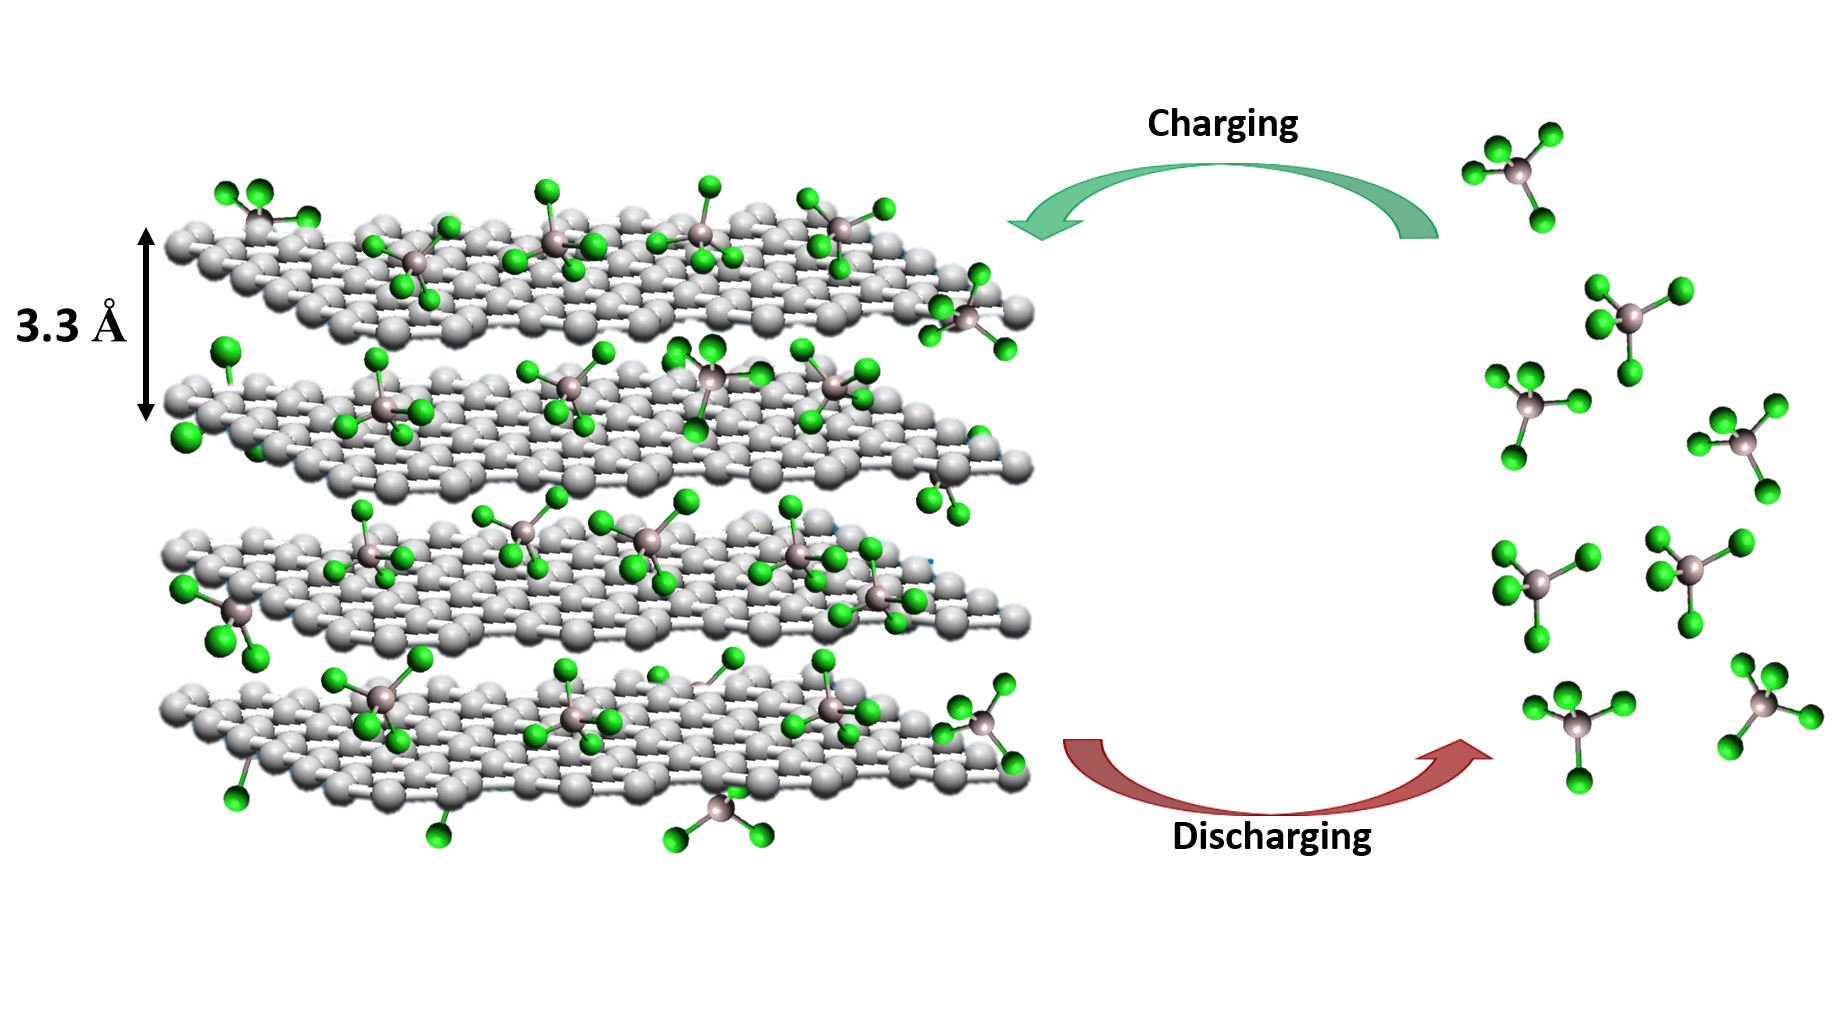
\includegraphics[width=\textwidth]{SF/graphitemech}
    \caption{Intercalation of \ce{AlCl4-} ions while cell charging and deintercalation during discharge in a Al/graphite cell. The interlayer distance between two graphite sheets is 3.3 \AA.}
  \label{SF:graphitemech}
\end{figure}

In this study, we compared four carbon-based materials with carbonised natural products. Super-P carbon has been used consistently as an additive to overcome conductivity loss in the active electrode material (for example, when a polymer binder such as polyvinylidene fluoride (PVDF) is added to it). Using it as an active material, we tried to find if Super-P contributes any capacity of its own to the battery's specific capacity. Activated carbon from natural products like rice or wood have been previously used in super-capacitors \cite{hussain_development_2019, frackowiak_carbon_2001}. Also known as 'hierarchical porous carbons', these structures contained pores of various sizes (mesopores and micropores), which enhanced the charge storage capacity by increasing the surface area of the electrodes. The pores absorb the charge carriers reversibly on their surface. Based on this hypothesis, we used activated carbon from human hair and hemp fibers as cathodes. 

\section{Results and discussion}

\begin{table}[tbh!]
\caption{Comparing average battery metrics of carbon cathodes} \label{table1}
\begin{center}
\begin{tabular}{|lcccc|}
\hline
Active material & {\textbf{Size}} & {\textbf{Specific capacity}} & {\textbf{Cell efficiency}} & {\textbf{Cell voltage}}\\
 & {\textbf{(pore size)}} & {\textbf{(mAh g$^{-1}$)}} & {\textbf{(\%)}} & {\textbf{(V)}}\\
\hline
Human hair & 5${\mu}$ m & 102 & 97 & 1.9 \\
Fullerene mix & 8.8 \AA & 78 & 85 & 1.7 \\
Hemp fibers & 2.3 $\mu$ m & 49 & 75 & 1.8 \\
SPCB & 300 \AA & 46 & 40 & 1.5 \\
\hline  % Please only put a hline at the end of the table
\end{tabular}
\end{center}
\end{table}

\begin{figure}[tbh!]
  \centering
  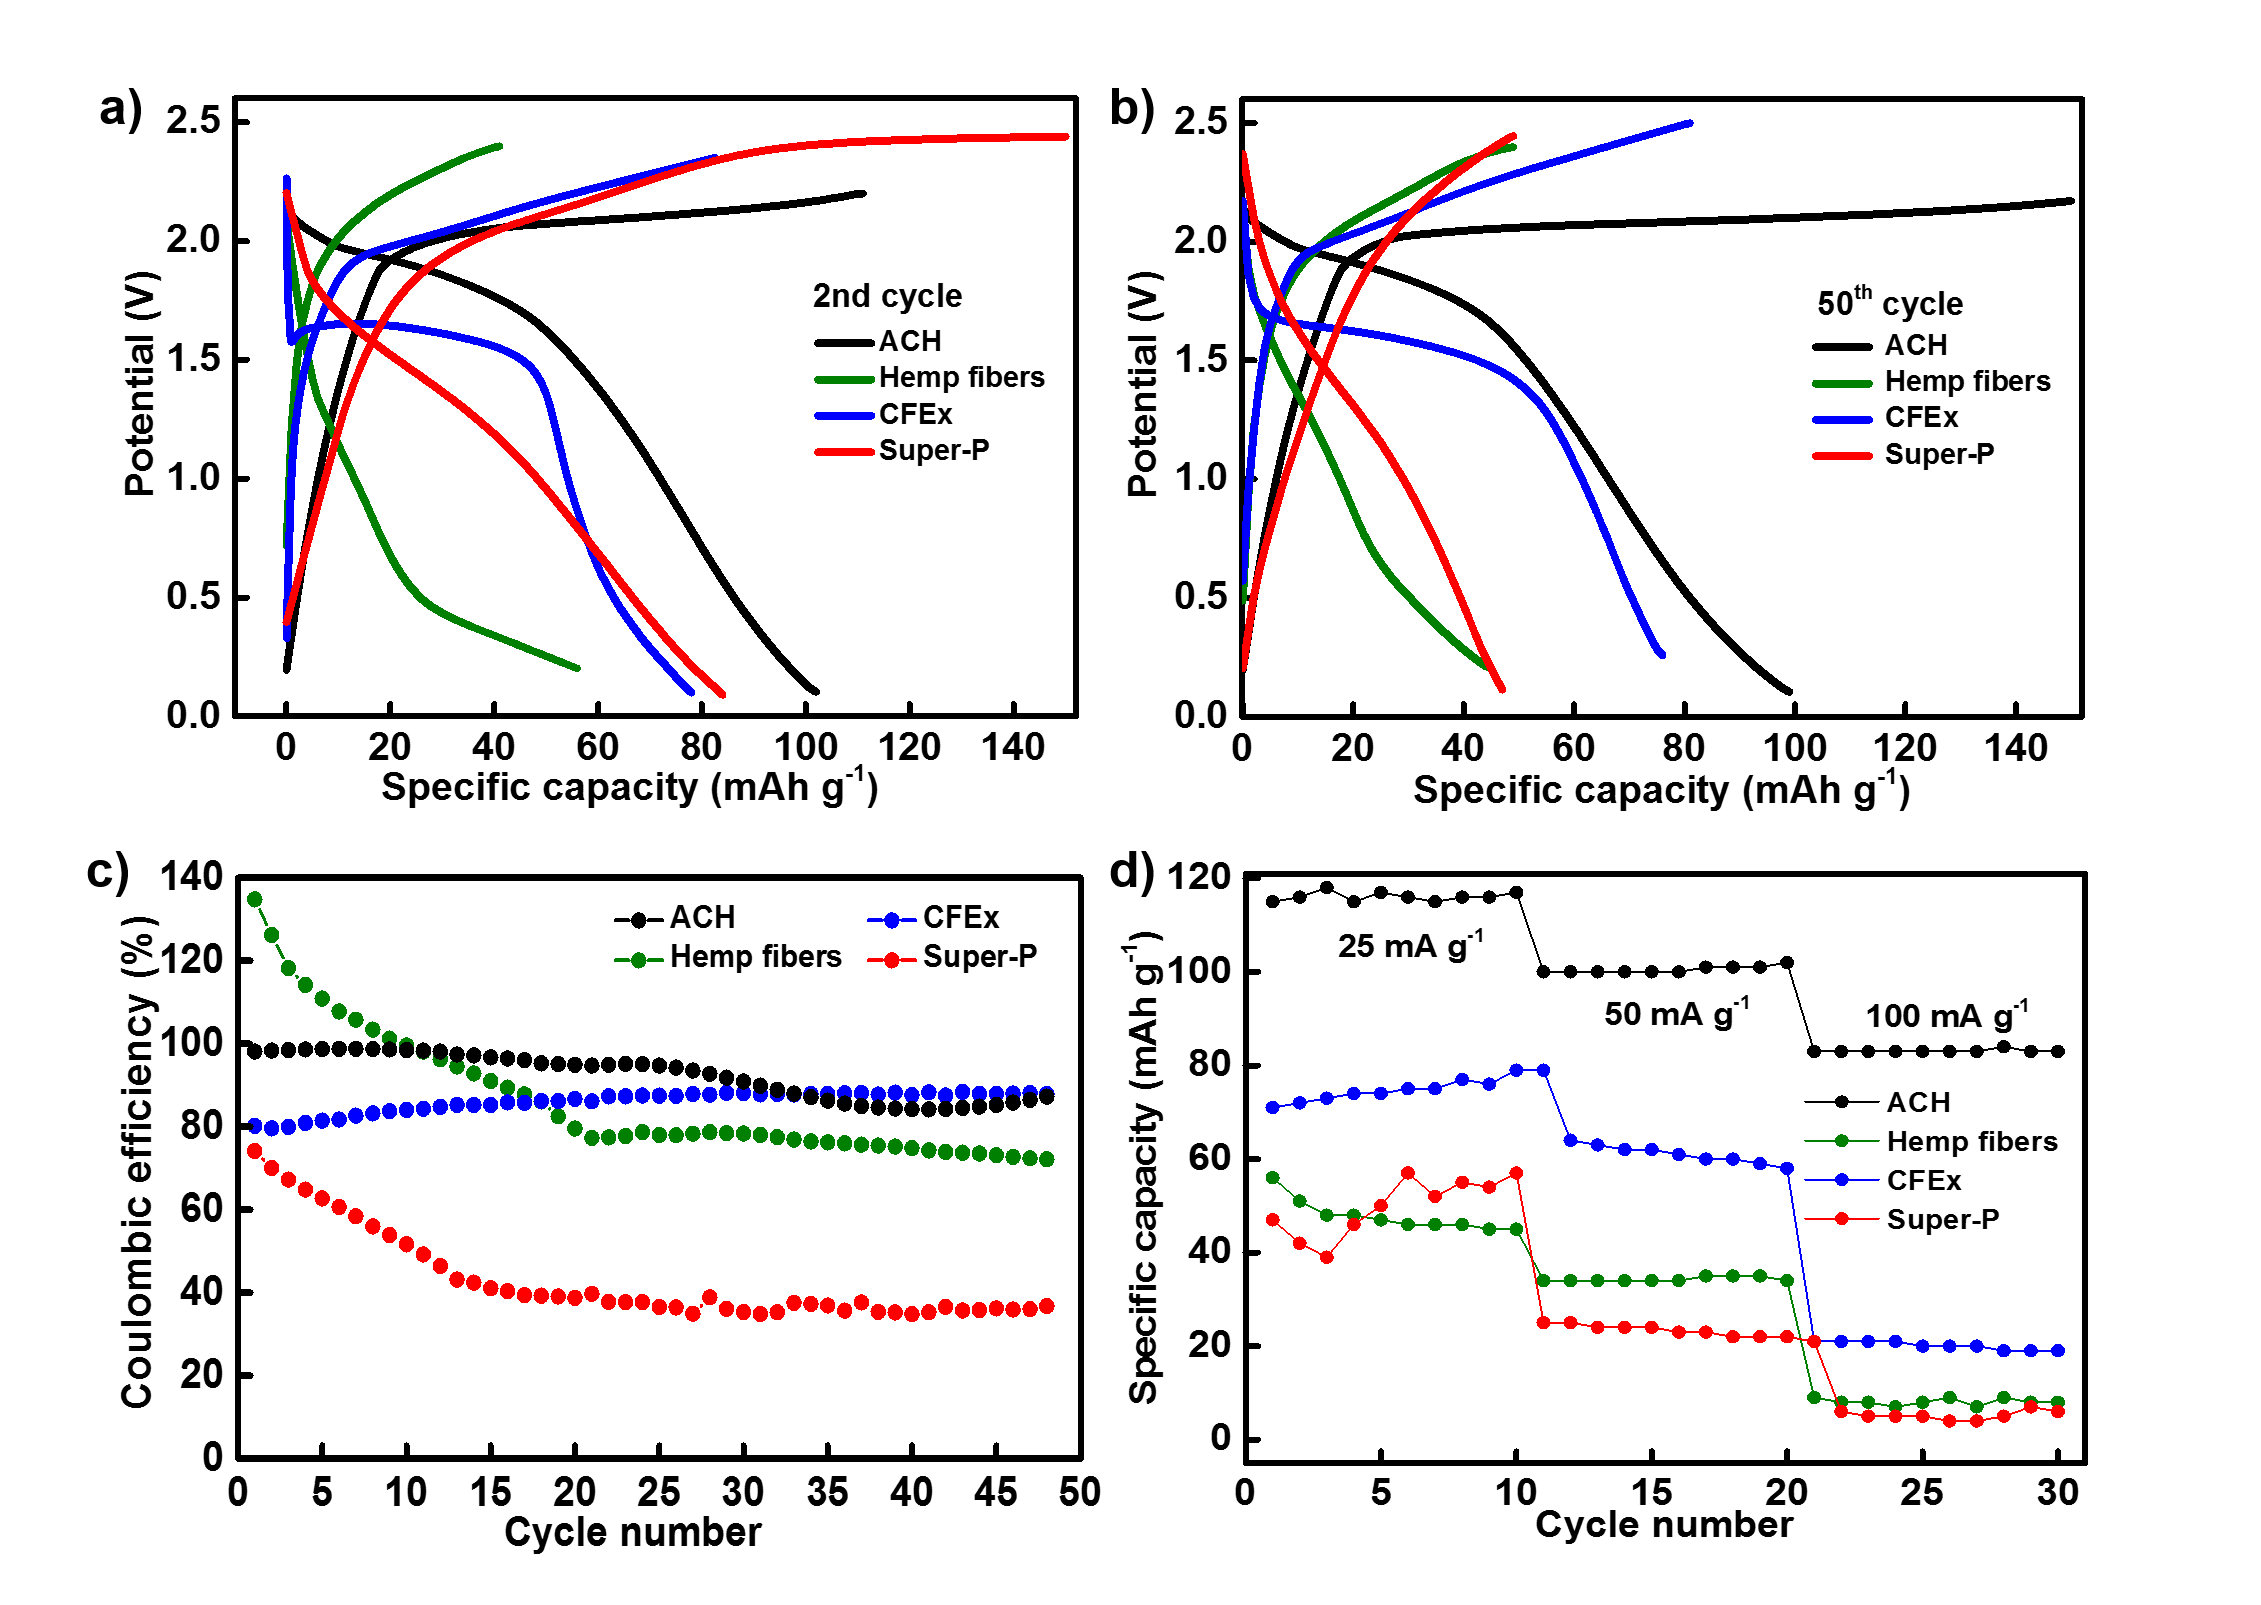
\includegraphics[width=\textwidth]{figures/CDCall}
    \caption{Specific capacities in the a) 1$^{st}$ and b) 50$^{th}$ cycle of human hair, hemp fiber, CFEx and SPCB cathodes at a current rate of 50 mA g$^{-1}$. c) Cell efficiencies of cells at a current rate of 50 mAg$^{-1}$. d) Specific capacities of carbon cells at current rates of 25 mAg$^{-1}$, 50 mAg$^{-1}$ and 100 mAg$^{-1}$ in a two-electrode setup against Al$^{3+}$/Al. }
  \label{figures:CDCall}
\end{figure}

Our battery system comprised a cathode, 99\% pure aluminium foil as an anode, and a room temperature ionic liquid (RTIL) acting as the electrolyte. ACH, hemp fibers and Super-P had an amorphous structure, however Raman spectra confirmed the presence of a few graphitic planes. Any number of graphite-like layers would allow \ce{AlCl4-} ions to intercalate when the cell was charged. However, CFEx, a mixture of \ce{C60} and \ce{C70} fullerenes, had crystalline character. Intercalation of aluminium into the fullerene cages was not observed. We suggest that \ce{AlCl4-} anions migrated through the gaps present in between fullerenes without altering the molecular structure. Using a \textit{Neware BTS 3000} battery analyser, specific capacities of the cathodes were recorded at a constant current density of 50 mA g$^{-1}$ (cf.\ Figure \ref{figures:CDCall}a and b). Structural changes in the cathode before and after the cycles were studied using Raman spectra, XRD spectra and scanning electron microscopy (SEM) images.

Figure \ref{figures:CDCall}a and b compares the specific capacities of all cells recorded in their 1$^{st}$ and 50${^th}$ cycles. Cells made of human hair displayed the highest capacity at around 100 mAh g$^{-1}$ with a coulombic efficiency at $\sim$95$\%$. High surface area due to the porous structure of the materials might have led to a additional 'capacitor-like' charge storage \cite{frackowiak_carbon_2001}. Hemp cells displayed a capacity of 56 mAh g$^{-1}$ in their first cycle, which decreased to 45 mAh g$^{-1}$ after 50 cycles. CFEx cells displayed a capacity of around 80 mAh g$^{-1}$ with a coulombic efficiency of $\sim$90\%. With an initial capacity of 84 mAh g$^{-1}$, specific capacity of SPCB cells decreased to 47 mAh g$^{-1}$ and a low coulombic efficiency at around 40\% was recorded. Capacity for SPCB and hemp cells decreased considerably after repeated charge/discharge cycles. A low coulombic efficiency (observed in both hemp and SPCB cells) can be attributed to parasitic reactions of the battery. These can include electrode or electrolyte interactions with impurities, or degradation of the cathode structure (pulverisation) \cite{gyenes}. However, capacity fade for CFEx and human hair cells was minimal. This suggest that CFEx and human hair have a more stable structure compared to hemp and SPCB and they store charge reversibly \cite{pramanick}. 

% In the above paragraph, you discuss 3 specific cells. This is suicidal (metaphorically speaking). In science you make a point by showing that something is reproducible. Having done just 3 expriments is asking for the reviewer to knock it down. You need to re-write this in a more general manner.

The production of activated carbon consists of carbonisation of a precursor at a temperature below 900$^{\circ}$ C in an inert atmosphere and chemical or physical activation of the carbonized precursor. Activating agents play an important role in determining the porosity of an activated carbon \cite{arenas}. Using alkali hydroxides, such as sodium and potassium hydroxide at high temperature creates micropores which increases the surface area of the material \cite{dong_commercial_2019, liu_hair-based_2017}. In this work, sodium hydroxide (NaOH) was used as the activating agent. The reaction that takes place inside the matrix after adding NaOH is:

\begin{center}
    4NaOH + C $\longrightarrow$ 4Na + 4\ce{CO2} + 2\ce{H2O} \cite{satish}
\end{center}

NaOH was reduced to free metal, Na, these atoms in turn expanded the carbon matrix after intercalating into the carbon structure. Increased temperature ($\sim$900$^{\circ}$ C) forces the  atoms out of the carbon matrix, thus creating micropores. Oxidation of carbon from oxygen atoms of the hydroxide group forms \ce{CO2} providing routes for channeling the Na atoms into the internal structure leading to well-connected porous structure \cite{satish}. The calcinating temperature used here was 750$^{\circ}$ C. Figure \ref{SF:ACHsyn} displays the flowchart for activated carbon synthesis. 

% Paragraph above: you need to prove/reason every statement that you make. You just claim a lot of stuff without providing any evidence. Also: ARTICLES!!!!!

%Unfortunately the structural domains appeared to have been damaged after this process. This phenomena negatively impacted its charge-storing capacity.  

% Above paragraph: Lots of unnecerssary information (see comments). Focus on what is relevant. Also sentences like the Carbon Valley one are suicidal. When you write, always have your worst scientific enemy in mind and write it so that you win.

Fullerenes have a fused-ring structure with a nucleus-to-nucleus diameter of 7.1\AA\ and a van der Waals diameter of 11 \AA in a single crystal. However, they are zero-dimensional materials, which means they cannot provide an efficient path for electron transport or long-range conductivity \cite{loutfy_fullerene_2002, winkler_two-component_2007}. They are known to be weak battery materials owing to their solubility in electrolytes, especially in LIBs \cite{seger_prospects_1991}. To test their solubility in \ce{AlCl3}-EMImCl, 100 mg of CFEx was mixed in the electrolyte and stirred for 24 hours. The solution was left to stand for another 24 hours inside a \ce{N2}-filled glove box. CFEx seemed to dissolve in our electrolyte (Figure \ref{SF:CFExsol} since no phase separation was observed. It has been reported that poly-sulphides formed during cycling in a lithium-sulfur battery, are soluble in the electrolyte. They form an insulating layer of \ce{Li2S} on the anode, which results in capacity fading \cite{sun_effect_2017}. Since no such effect was observed in aluminium-fullerene cells, this phenomena does not seem to impact the charge-storing capacity of CFEx. On the contrary, the cells displayed excellent capacity retention at various current rates(Figure \ref{figures:CDCall}d).   

 \begin{figure}[tbh!]
  \centering
  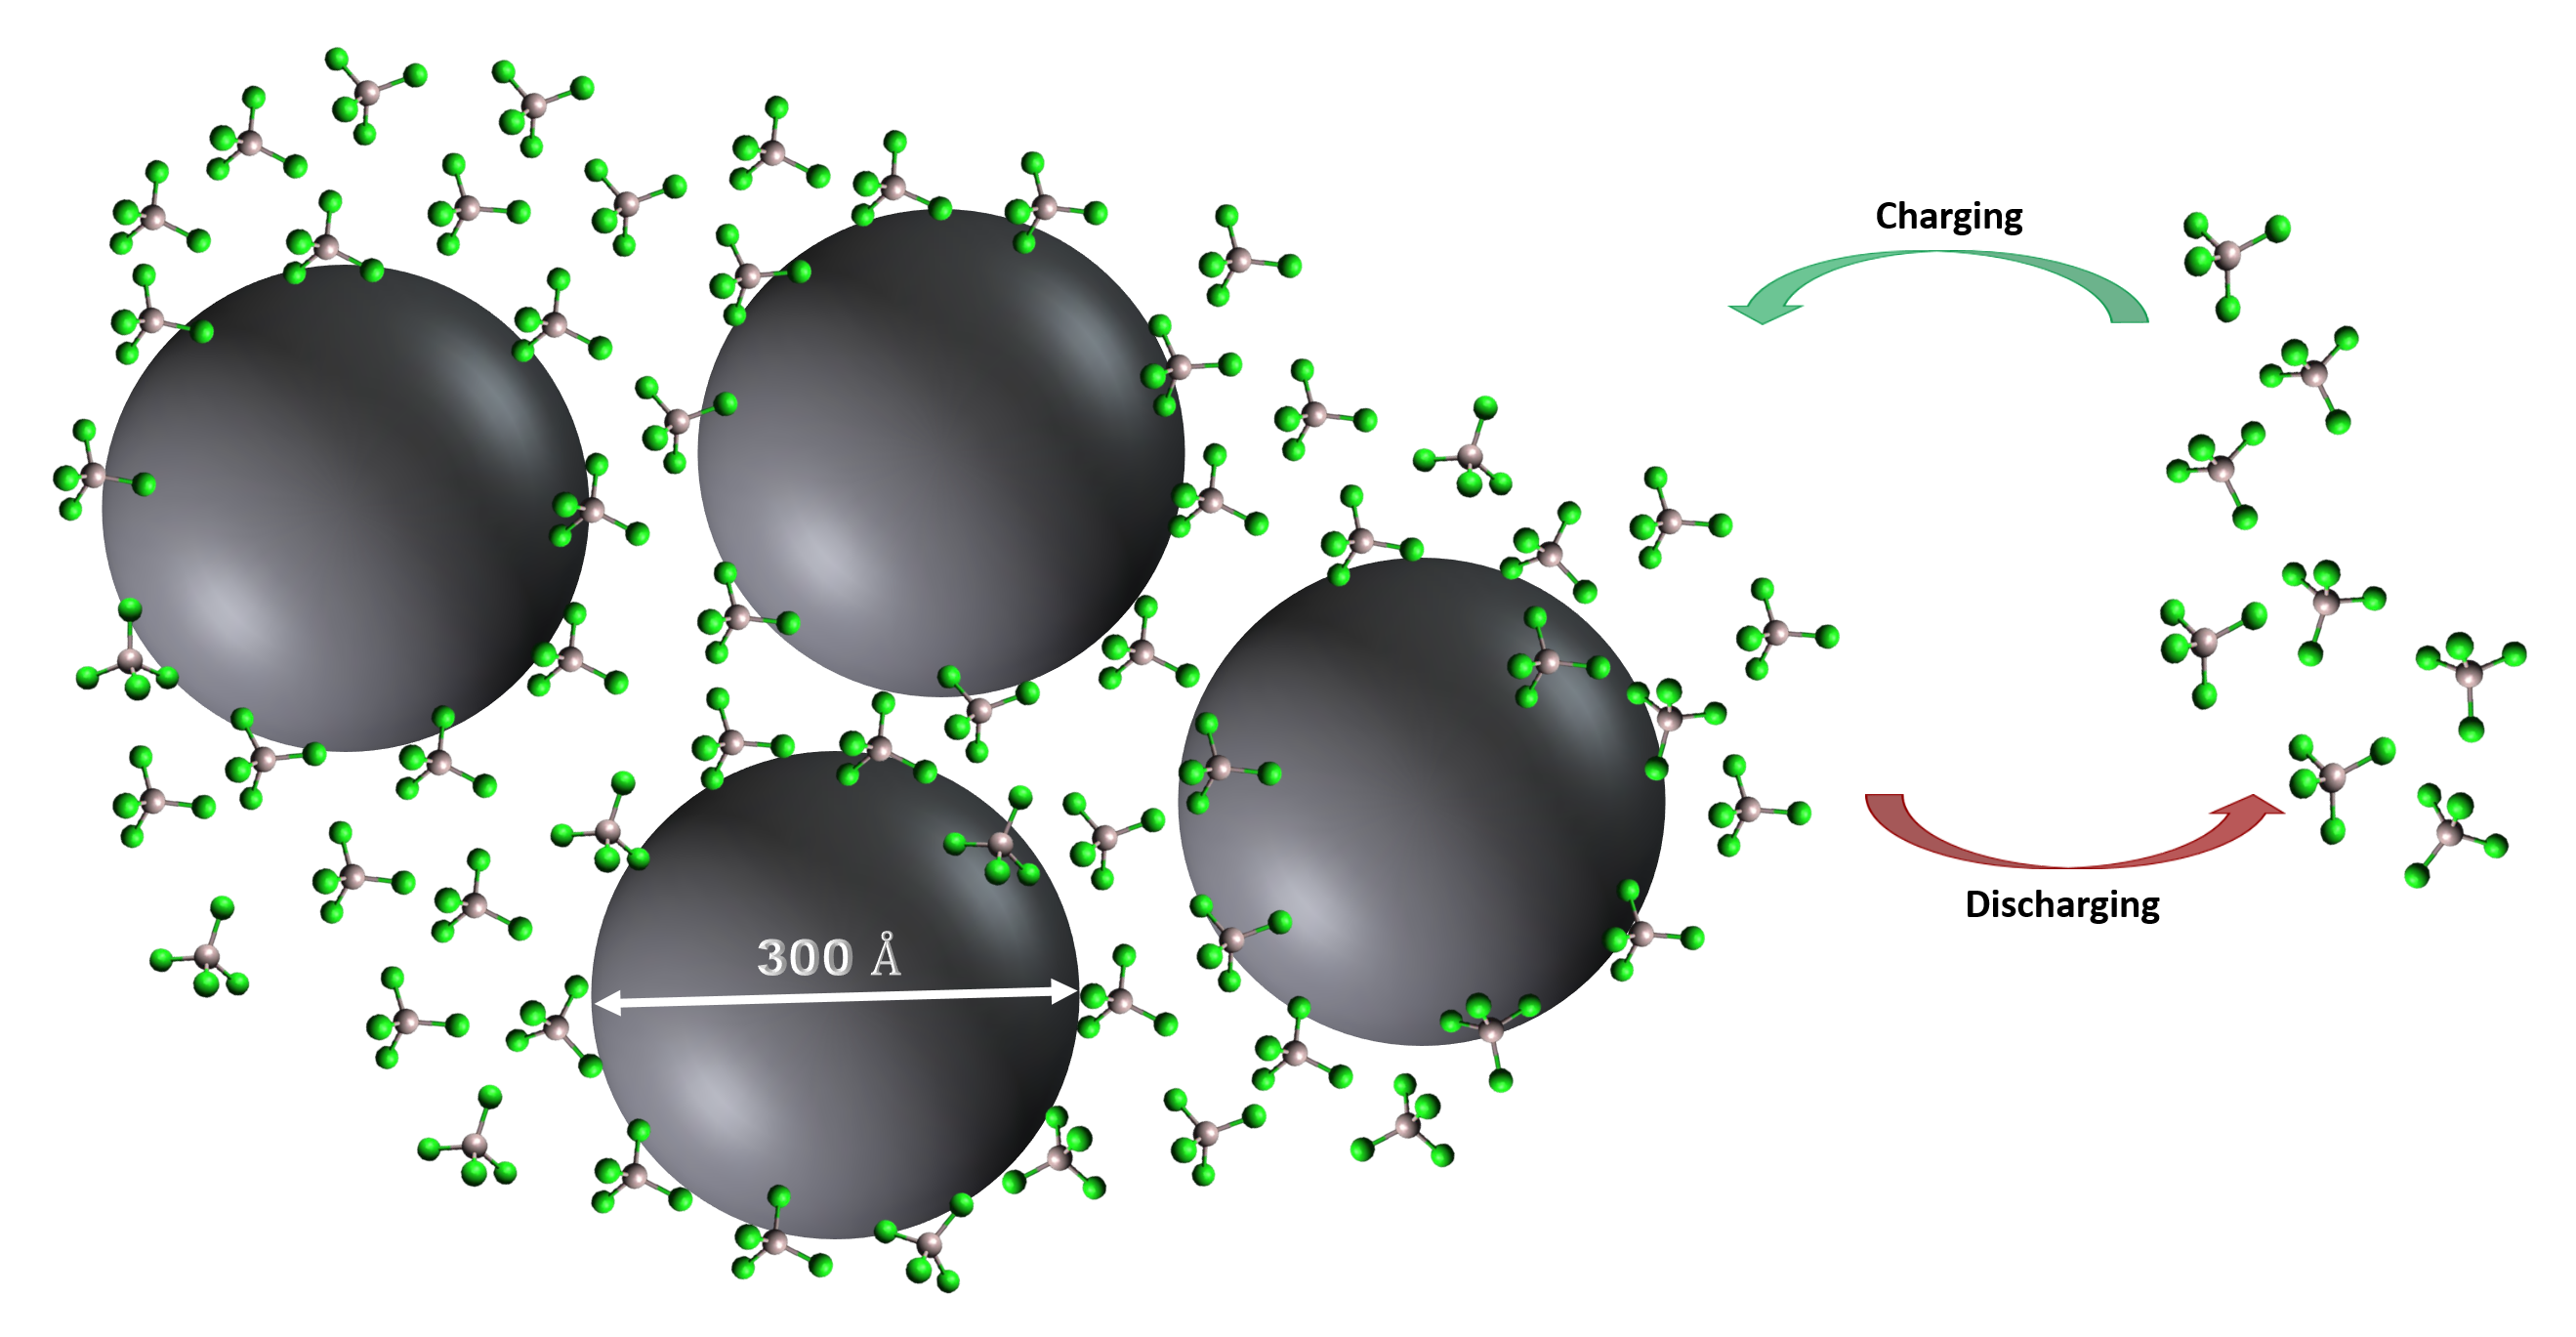
\includegraphics[width=\textwidth]{figures/superPmech}
    \caption{Suggested mechanism for a \textbf{Al/Super-P} cell. Super-P has a very amorphous structure with a few graphite-like planes present in it. \ce{AlCl4-} ions intercalate into those layers and give the cell its capacity. However, cathode pulverisation results in capacity fading.}
  \label{figures:superPmech}
\end{figure}

Super-P is an amorphous form of carbon with a high surface area of 62 m$^2$ g$^{-1}$ and a highly disordered structure. Its pore size ranges from $\sim$30-50 nm \cite{younesi_analysis_2015}. SPCB has the least graphitic structure if compared to human hair and hemp fibers. It seems continuous cycling might have destroyed the arrangement of the carbon atoms, which resulted in poor capacity retention and low coulombic efficiencies.

 \begin{figure}[tbh!]
  \centering
  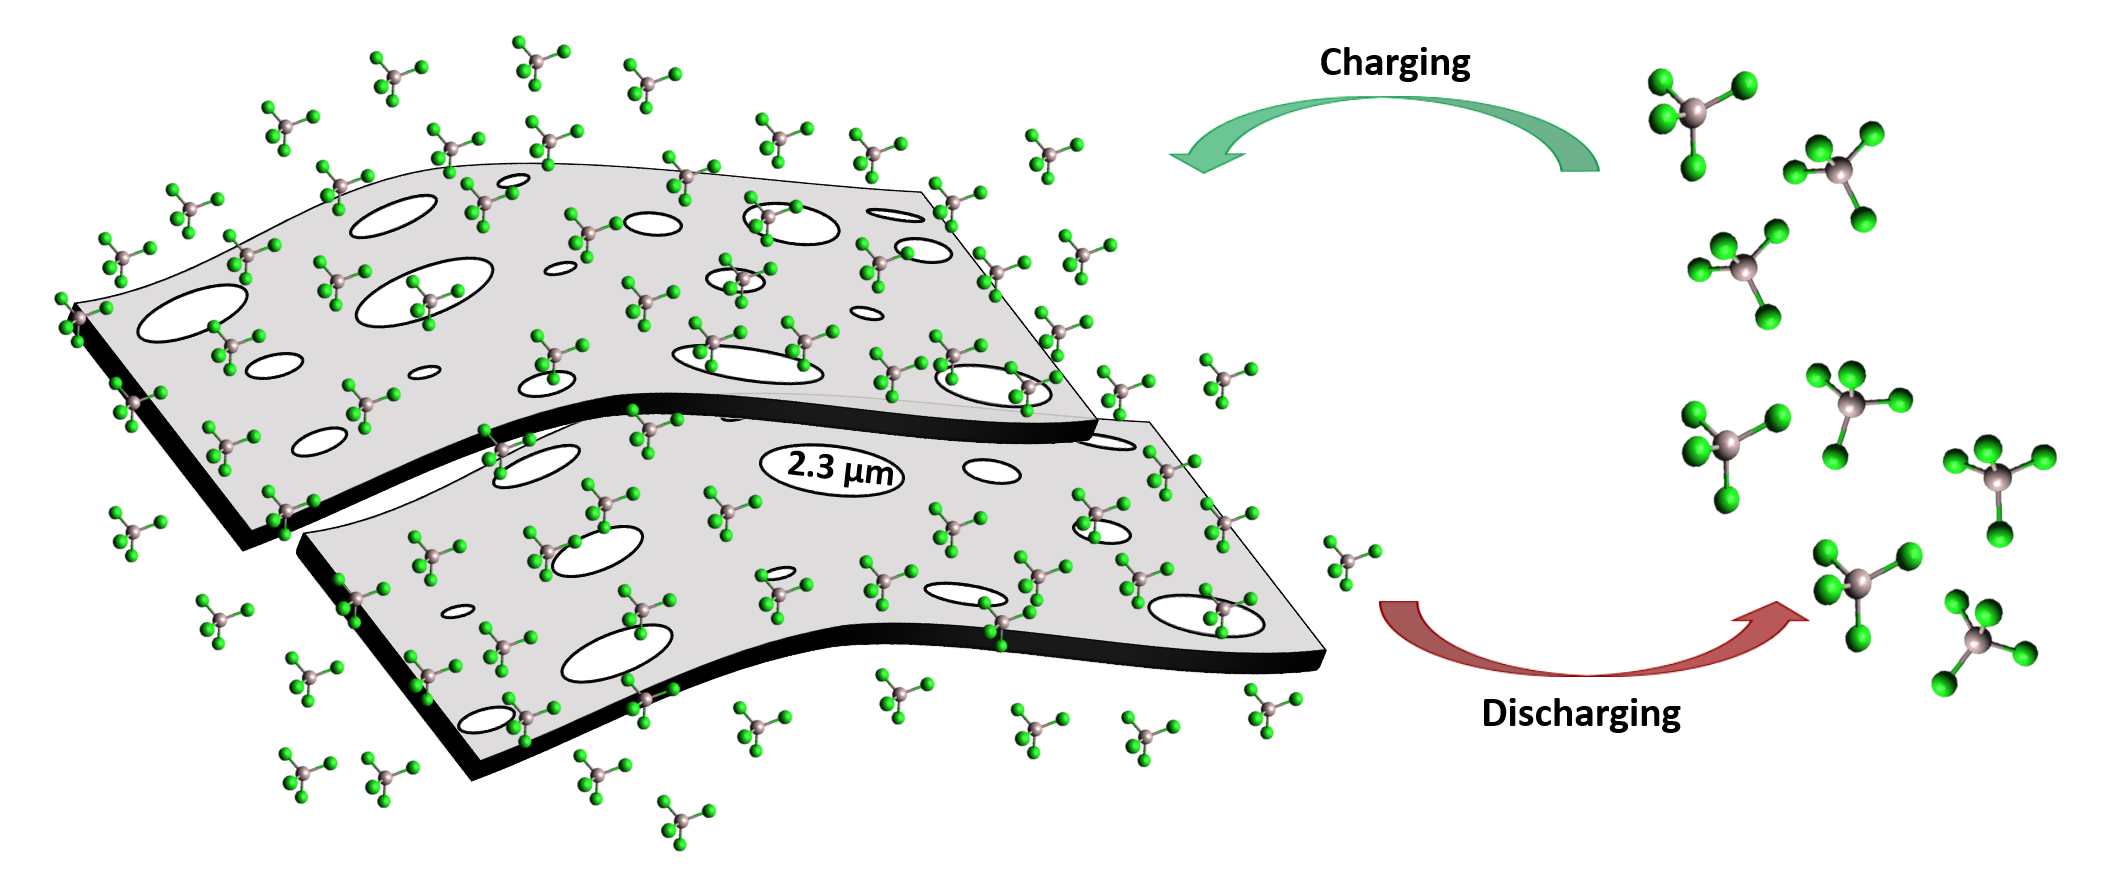
\includegraphics[width=\textwidth]{figures/hempmech}
    \caption{Suggested mechanism for a \textbf{Al/hemp} cell. The fibers have a large pore size (2.0-2.5 $\mu$m) which allow the \ce{AlCl4-} to get absorbed on the cathode surface but agglomeration of carbon atoms after a few cycles reduces the active sites available for charge storage, which reduces cell's capacity after every cycle.}
  \label{figures:hempmech}
\end{figure}

 \begin{figure}[tbh!]
  \centering
  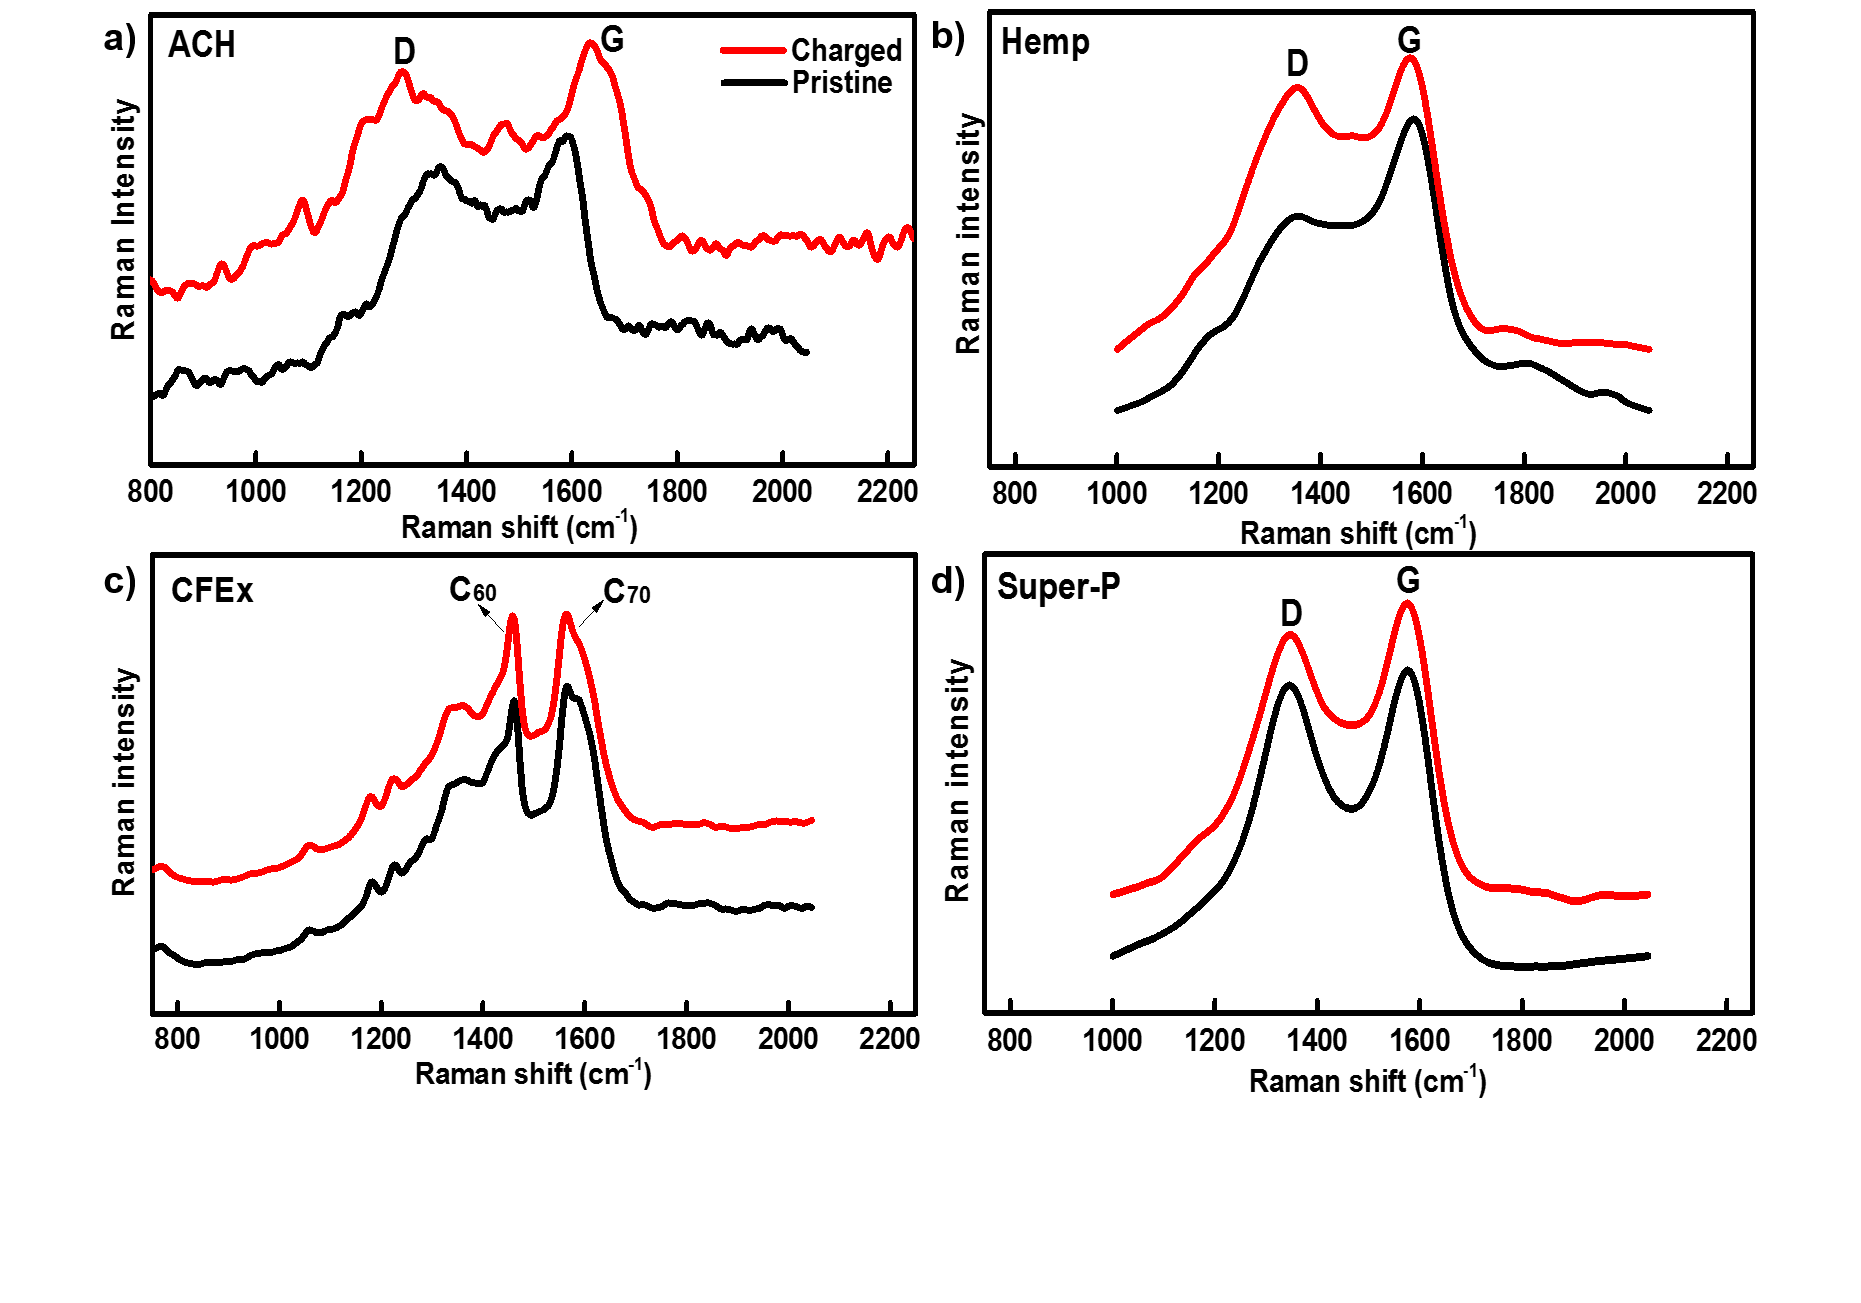
\includegraphics[width=\textwidth]{figures/raman}
    \caption{Raman spectra of pristine (in black) and charged (in red) a) CFEx , b) hemp fibers, c) ACH and d) Super-P cathodes indicating presence of both D and G-bands.}
  \label{figures:raman}
\end{figure}

In aluminum-graphite cells, it has been established that \ce{AlCl4-} ions intercalate while charging \cite{lin_ultrafast_2015}. Since the materials we tested have graphitic planes present, we focused our analysis on the pristine and charged electrodes. Figure \ref{figures:raman} displays Raman spectra of the tested cathodes. Pristine human hair, hemp fibers and SPCB had a significant D-band present indicating absence of an ordered structure with presence of lattice defects and deformities (at $\sim$1300 cm$^{-1}$ for human hair, 1329.7 cm$^{-1}$ for hemp fibers, and 1352.0 cm$^{-1}$ for SPCB). Figure \ref{figures:raman}c displayed the characteristic features of both \ce{C60} and \ce{C70} molecules. The 'pentagonal pinch mode', which is usually observed in a \ce{C60} Raman spectrum, was present at 1460 cm$^{-1}$. However, \ce{C70} has multiple bands. Reduction in its molecular symmetry increases the number of vibrational modes, thus increasing the active Raman bands \cite{kimbrell_analysis_2014}. Pristine CFEx cathode was composed of both \ce{C60} and \ce{C70} Raman bands as seen in Figure \ref{figures:raman}c. It was interesting to note that charged CFEx cathodes looked strikingly similar. Since Raman spectroscopy is sensitive to minute differences in the molecular morphology, results suggested that the structure remained intact after cycles. Human hair has a high surface area and an inter-connected mesoporosity. The charged cathodes showed a higher FWHM which suggests an increase in the lattice defects. Obviously, these defects arise after intercalation of chloroaluminates; it is assumed that these ions intercalate into the few graphitic planes present in the carbon matrix. In addition, a highly porous structure allows surface adsorption of charge carrying species (much like in super-capacitors) \cite{beguin_carbons_2014}. Intercalation into graphitic planes/micropores, along with surface adsorption of chloroaluminates, result in aluminium-hair batteries performing better than other materials by storing more charge\cite{brezesinski_ordered_2010}. A schematic of a possible mechanism is shown in Figure \ref{figures:ACHmech}.
%contains about 51\% carbon, 17\% nitrogen, 21\% oxygen, 6\% hydrogen, 5\% sulfur, and trace amounts of iron, magnesium, arsenic, chromium and various minerals \cite{lee_chemistry}.  
Hemp fibers and SPCB had fewer graphitic planes and a highly disordered structure to begin with. The lattice defects seemed to increase after galvanostatic cycles. Continuous intercalation or absorption of ions on their surface would have further destroyed the cathode structure. This might be the reason why hemp and SPCB cells failed to retain capacity after a few cycles. However, CFEx does not have graphitic planes. It consists of a bunch of \ce{C60} and \ce{C70} fullerenes. Insertion of \ce{AlCl4-} ions inside the cage-like structure would be thermodynamically impossible. Since the fullerenes have a very high surface area, surface adsorption of ions is likely \cite{adams}. Furthermore, it might be possible for the anions to seep through the gaps present in between two fullerenes \ref{figures:CFExmech}. Capacity retention of the aluminium-CFEx cells suggests that the interaction between the fullerenes and \ce{AlCl4-} ions takes place in a systematic way.

\begin{figure}[tbh!]
  \centering
  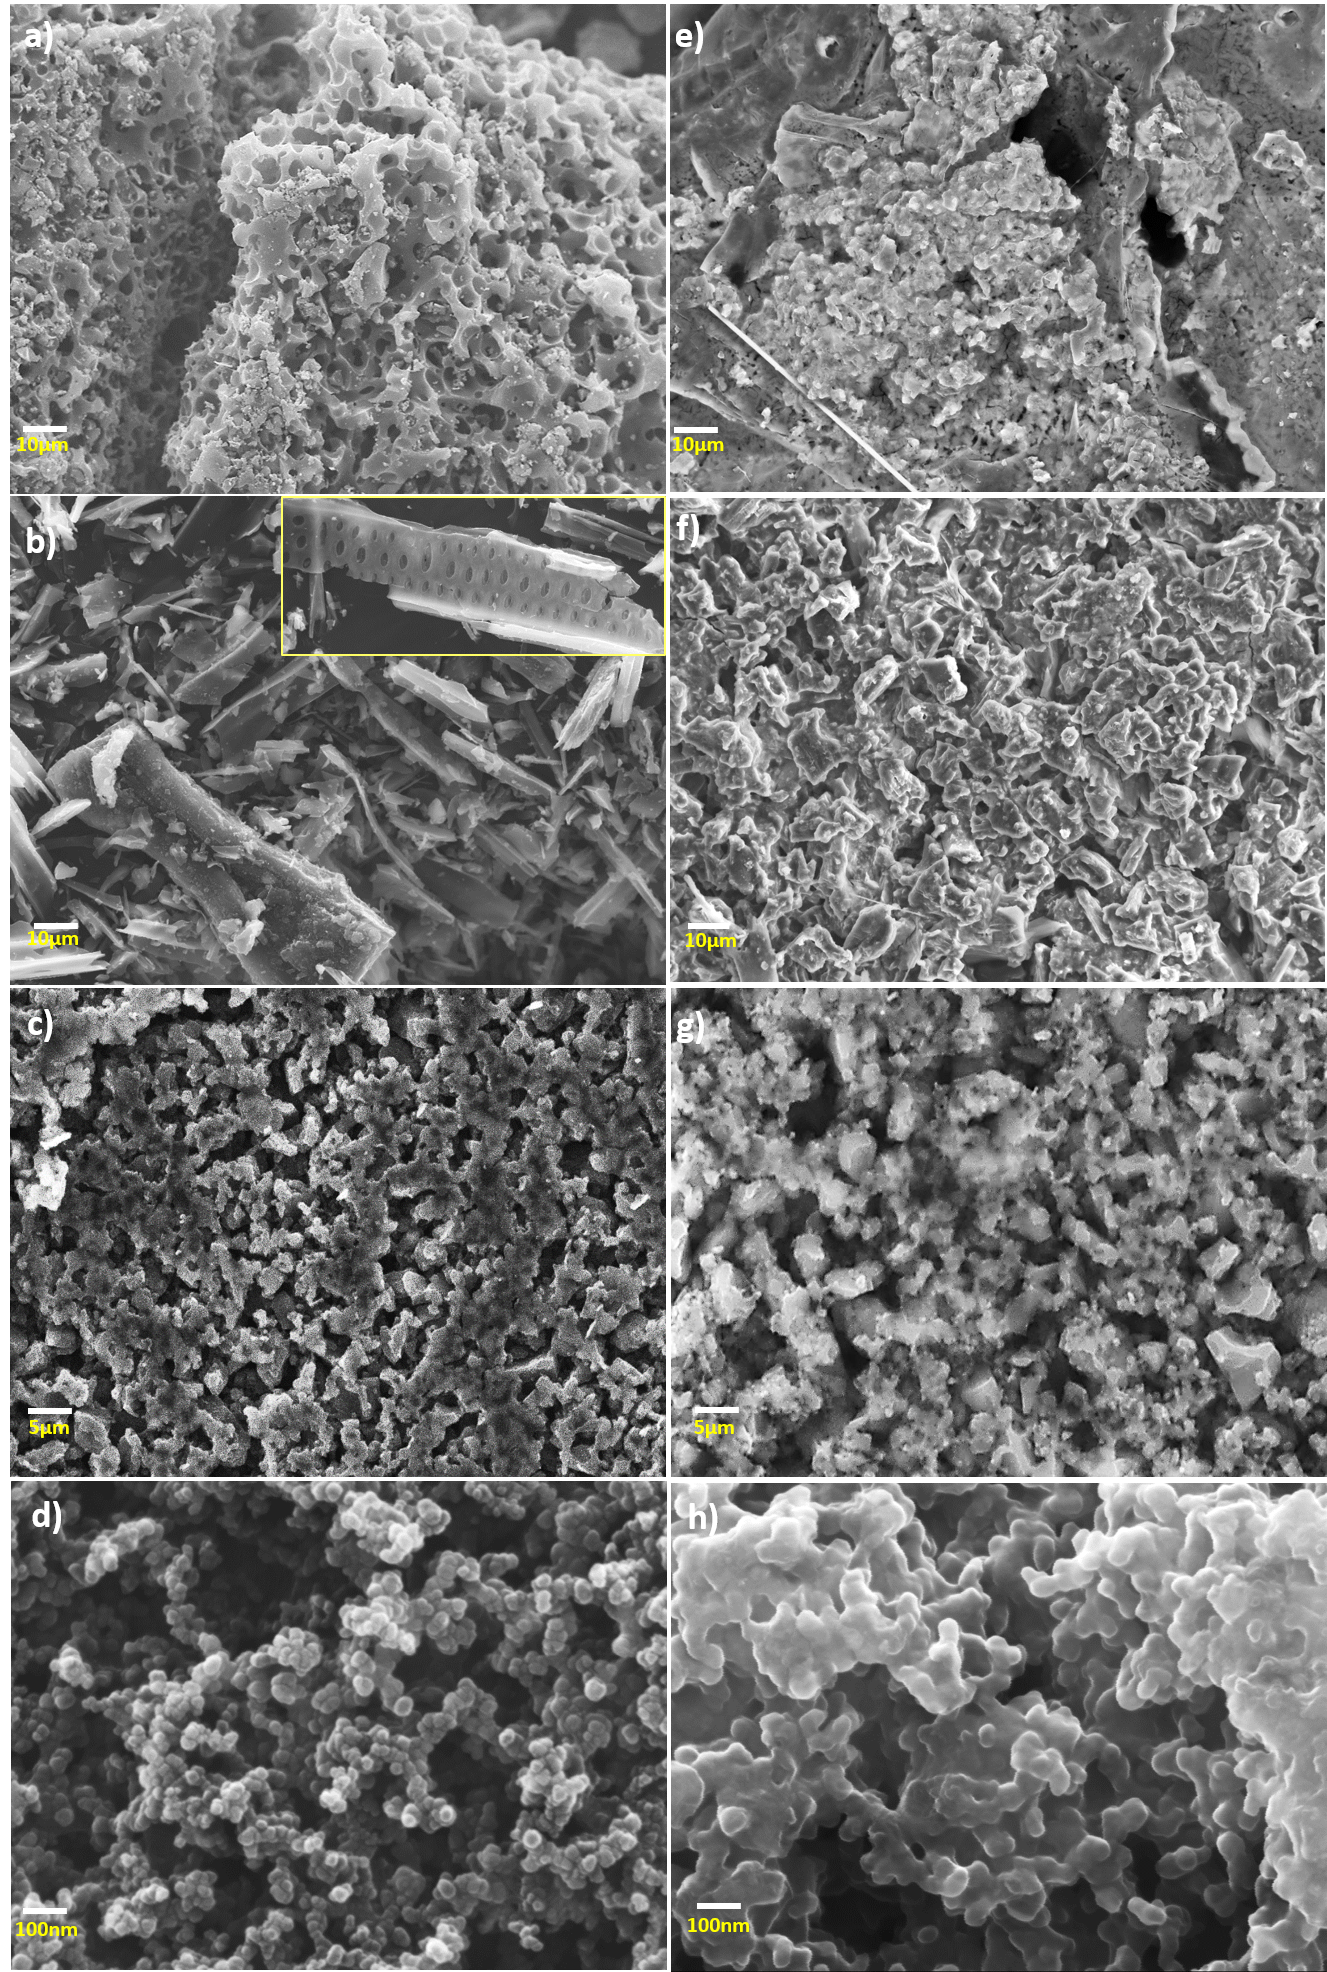
\includegraphics[width=\textwidth]{figures/SEM}
    \caption{Scanning electron microscopy images comparing pristine a) ACH, b) hemp fibers, c) CFEx and d) Super-P; and charged e)ACH, f) hemp fibers, g) CFEx and h) Super-P electrodes. Hemp fibers and Super-P undergo prominent changes after charge/discharge cycles (visible agglomeration of carbon atoms).}
  \label{figures:SEM}
\end{figure}

In Figure \ref{figures:SEM}, we compared the SEM images of pristine (Figure \ref{figures:SEM}a, b, c and d) and charged (\ref{figures:SEM}e,f,g and h) cathodes of all tested materials. Hemp and SPCB had a porous structure (Figure \ref{figures:SEM}b and d) to begin with, which degraded after a few cycles (Figure \ref{figures:SEM}f and h). Significant agglomeration occurred in hemp and SPCB cathodes after continuous cycling.  

\begin{figure}[tbh!]
  \centering
  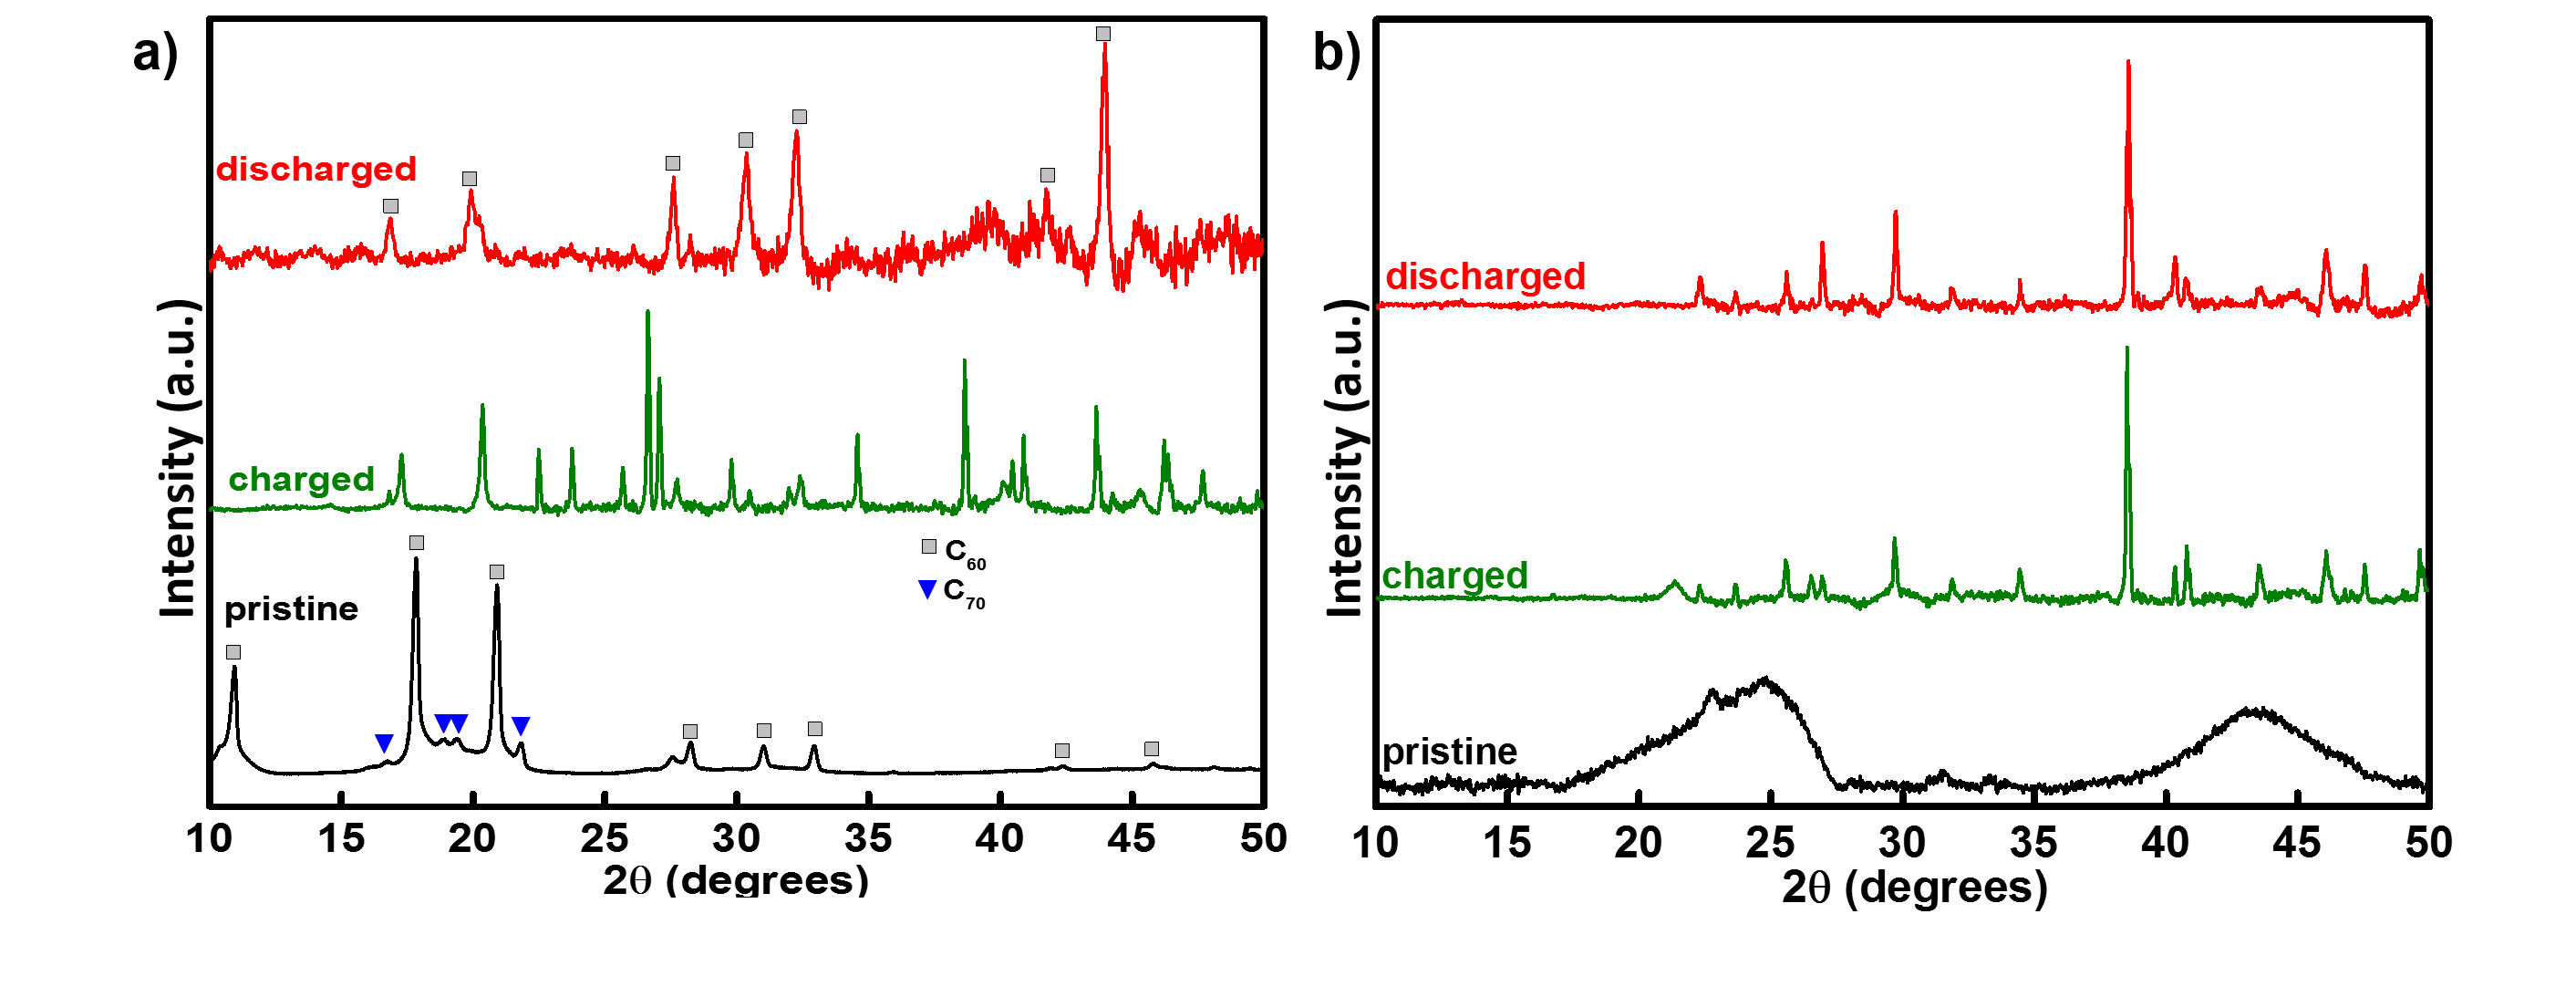
\includegraphics[width=\textwidth]{figures/XRD}
    \caption{XRD spectra comparing a pristine (black), charged (green) and discharged (red) a) CFEx and b)ACH cathode to study changes in their lattice after 50 galvanostatic cycles in a two-electrode setup against \ce{Al$^{3+}$/Al} with characteristic peaks marked for \ce{C60} (in grey) and \ce{C70} (in blue).}
  \label{figures:XRD}
\end{figure}

To fully understand the mechanism in CFEx and human hair, we examined their XRD spectra in Figure \ref{figures:XRD}. Pristine, charged and discharged cathodes of CFEx and human hair were compared in Figure \ref{figures:XRD}a and b respectively. Pristine cathodes displayed the characteristic peaks of both \ce{C60} and \ce{C70} at 2$\theta$ values of 10.9$^{\circ}$, 17.8$^{\circ}$, 20.9$^{\circ}$ and 28.2$^{\circ}$ for \ce{C60} and 18.9$^{\circ}$, 19.3$^{\circ}$ and 21.8$^{\circ}$ for \ce{C70} molecules. Charged electrodes displayed new diffraction peaks at lower 2$\theta$ values. However, after discharge, the XRD pattern resembled the pristine cathode. This data strongly suggests a reversible process. To confirm, we calculated the unit cell lattice parameters for both pristine and charged cathodes for a \ce{C60} molecule. The unit cell had a tetragonal crystal system with space group of P42/mmc and a space group number 131 (ICDD: 04-013-1339 for \ce{C60}). Lattice parameter 'a' and 'b' for the charged electrode changed from 9.06 \AA to 9.57 \AA . Lattice parameter 'c' changed from 15.03 \AA to 15.65 \AA, in Figure \ref{figures:CFExcryst}a and b. Lattice parameters for discharged cathode were closer to pristine values. These changes suggested a reversible intercalation process taking place. A possible site for \ce{AlCl4-} intercalation is depicted in Figure \ref{figures:CFExcryst}c. XRD spectra for human hair cathodes was inconclusive (Figure \ref{figures:XRD}b). Pristine cathode showed broad peaks suggesting an amorphous and highly porous structure. However, the material became more ordered after cycles. Charged and discharged cathodes have similar patterns which means no structural changes took place in aluminium-hair batteries. Also, presence of crystallinity in an active material does not limit the surface-based charge storage \cite{kim_synthesis_2006, jow_factors_2018}. So, we hypothesise that human hair followed a capacitor-like behaviour after intercalation of ions in the initial cycles.

 \begin{figure}[tbh!]
  \centering
  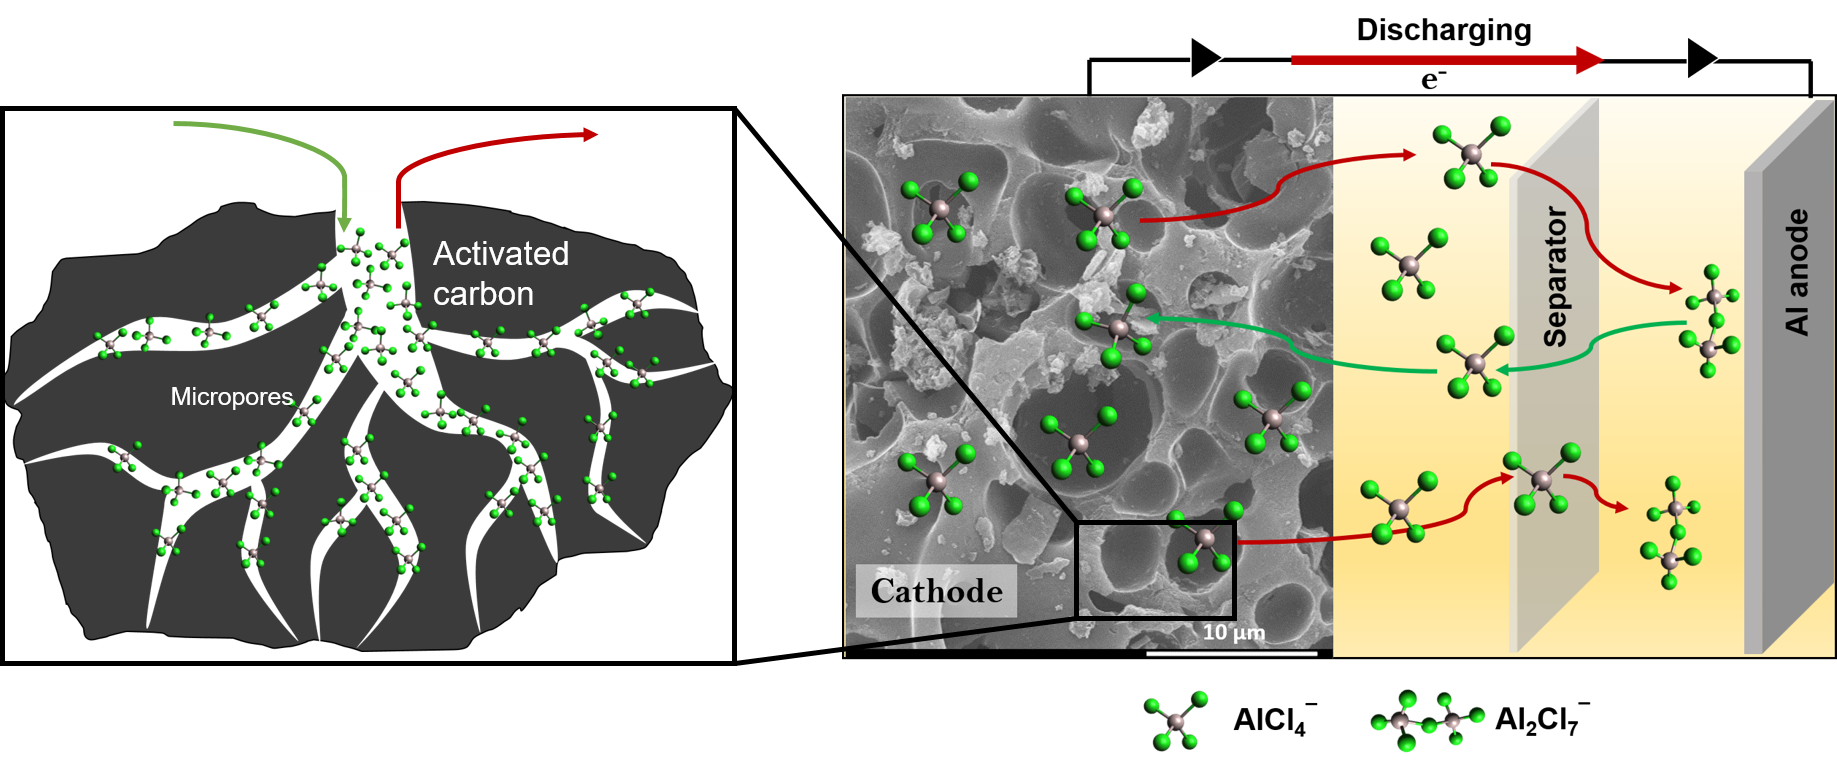
\includegraphics[width=\textwidth]{figures/ACHmech}
    \caption{Suggested mechanism for an aluminium-human hair cell.}
  \label{figures:ACHmech}
\end{figure}

\begin{figure}[tbh!]
  \centering
  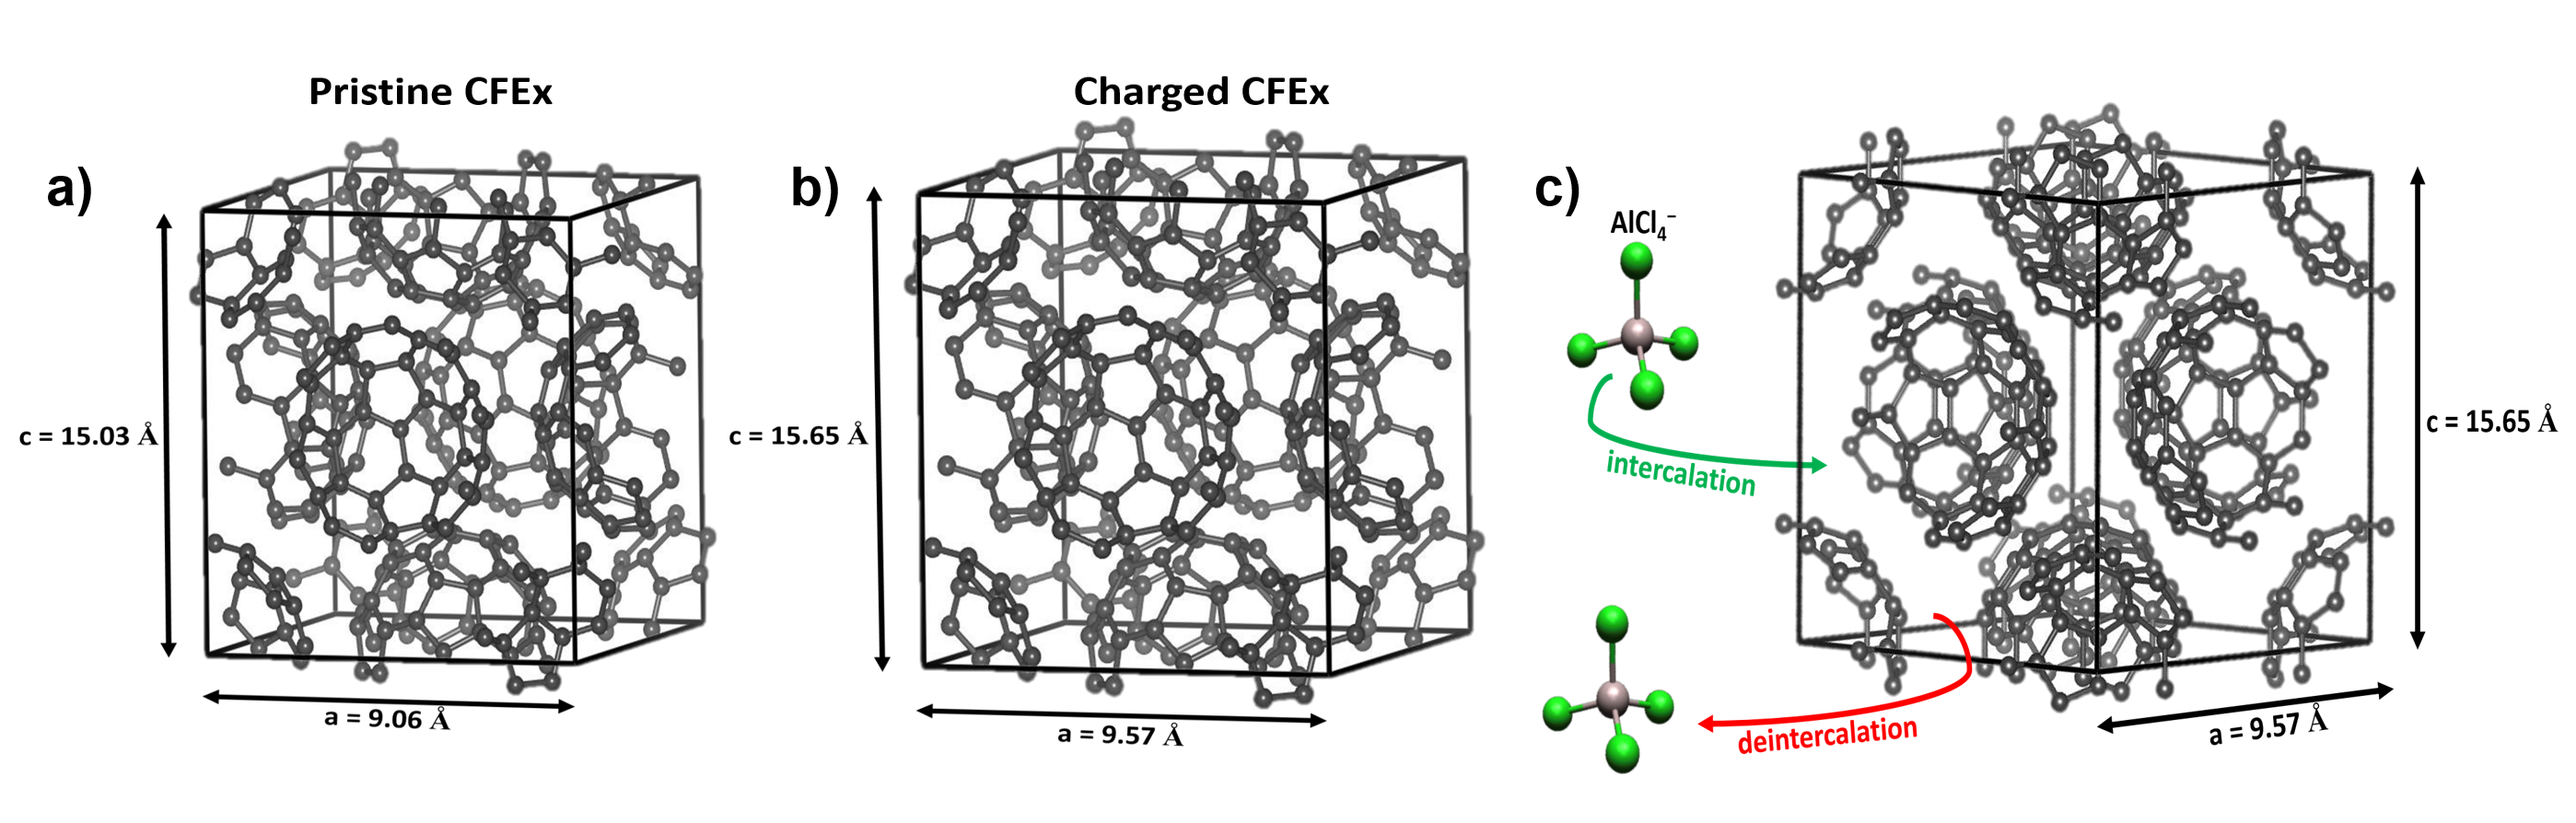
\includegraphics[width=\textwidth]{figures/CFExcryst}
    \caption{Changes in the lattice parameters of a \ce{C60} unit cell. a) Pristine \ce{C60}unit cell, b) charged \ce{C60}unit cell with increased parameters suggesting a uniform shift in the lattice after charge/discharge. c) Expected intercalation sites of \ce{AlCl4-} ions in the unit cell.}
  \label{figures:CFExcryst}
\end{figure}

%Charged Super-P and hemp fiber electrodes underwent degradation and appeared clumped together resulting in capacity decay. This was visible from their electrochemical results where a rapid decrease in capacity and cell efficiency was noted. 

%XPS analysis results... C 1s 
\begin{figure}[tbh!]
  \centering
  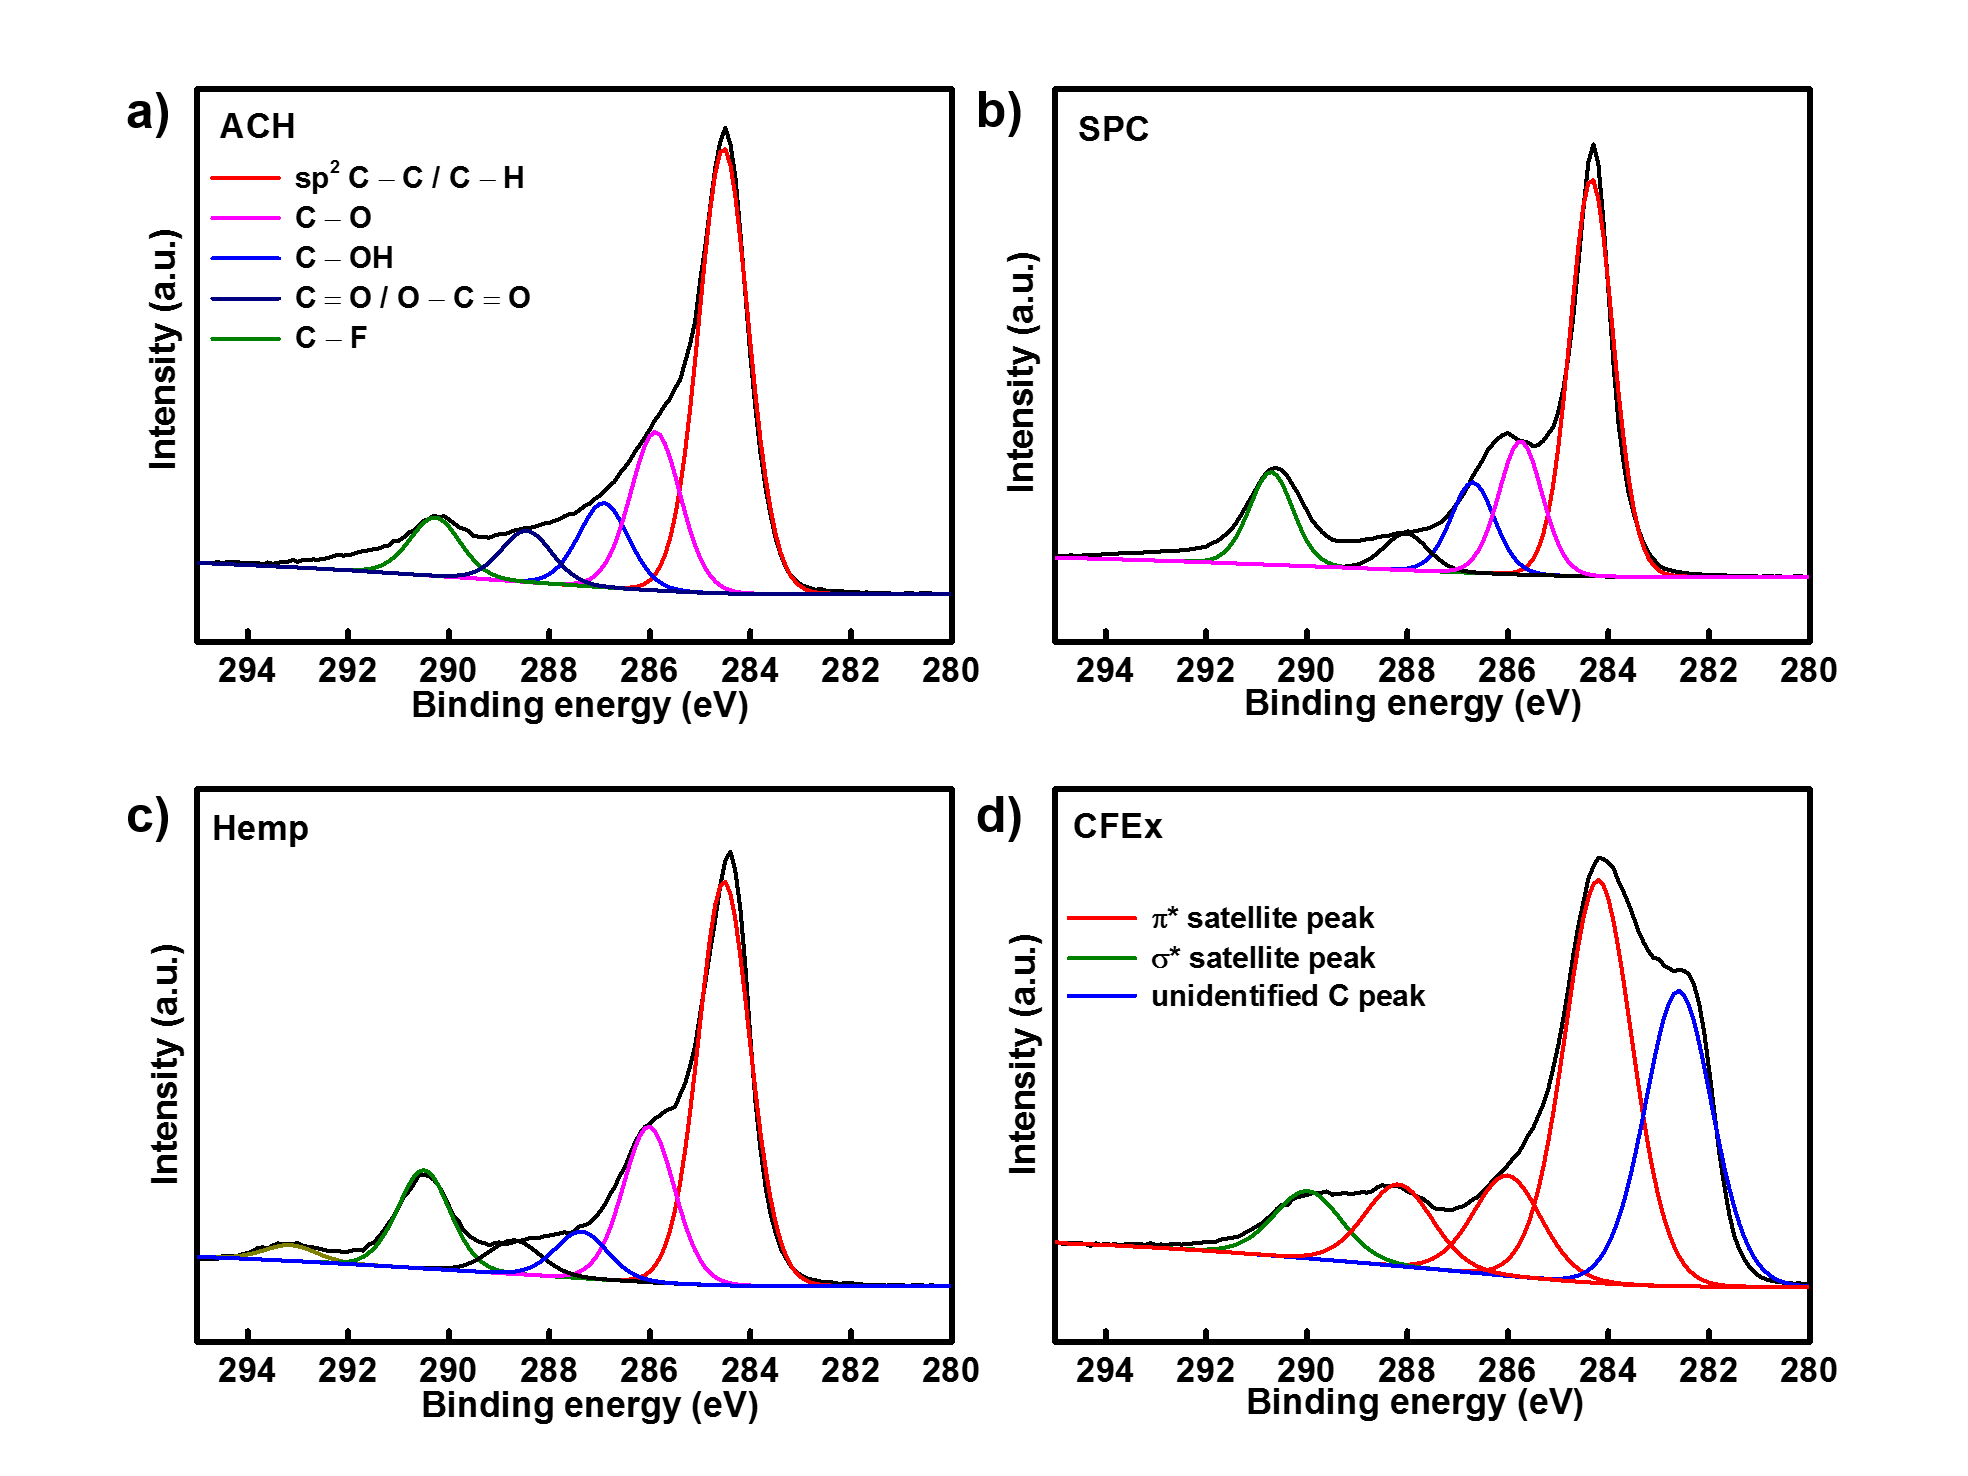
\includegraphics[width=\textwidth]{figures/XPSC}
    \caption{Carbon 1s XPS spectra of pristine a) ACH, b) Super-P, c) hemp fibers and d) CFEx cathodes.While ACH, Super-P and hemp fibers observe carbonyl functional groups, CFEx cathodes have symmetrical looking $\pi$* and $\sigma$* satellite peaks.}
  \label{figures:XPSC}
\end{figure}

We observed XPS spectra of all pristine cathodes to understand their composition. Human hair, hemp fibers and SPCB had similar looking peaks for carbon 1s orbital as shown in figure \ref{figures:XPSC}. Binding energies suggesting sp$^2$ C-C/ C-H, C-O/ C-OH, O-C=O/ C=O and C-F bonds (formed between the binder and active material) appeared in hair, hemp fibers and SPCB cathode spectra. Hair is mainly composed of a protein called keratin displayed in Figure \ref{SF:keratin} and the multiple chemical environments of carbon in Figure \ref{figures:XPSC}a) are derived from Keratin. Sulphide bonds are an essential part of this protein and a C-S binding energy is observed at 286.94 eV (blue peak).

\begin{table}
\caption{Carbon 1s peaks for various binding energies.} \label{table2}
\begin{tabular}{|cccccccc|}
\hline
Active & C-H/ & C-O/ & C=O/ & C-F & Pyrrolic N/ & aliphatic C-O & aromatic C=O\\
material & C-C & C-OH & O-C=O & & Pyridinic N & & \\
\hline
Human hair & 284.5 eV & 285.8 eV & 288.4 eV & 290.2 eV & 400.2 eV/ & 533.0 eV & 531.2 eV\\
& & & & & 398.3 eV & & \\
CFEx & 284.2 eV & 286.0 eV & 288.2 eV & 290.0 eV & 399.3 eV & 531.3 eV & 530.2 eV\\
Hemp fibers & 284.5 eV & 286.0 eV & 288.7 eV & 290.5 eV & 400.3 eV & 532.9 eV & 531.4 eV\\
SPCB & 284.3 eV & 286.7 eV & 288.0 eV & 290.7 eV & 400.2 eV & 532.8 eV & ---\\
\hline
\end{tabular}
\end{table}

Functional groups that contain oxygen, such as carbonyl and ester groups, improve the wettability of a material and increases the availability of active surface area \cite{younesi_analysis_2015}. SPCB is produced from partial oxidation of petrochemical precursors and exhibits a large specific surface area with a very high electrical conductivity \cite{gnanamuthu_electrochemical_2011}. A perfect graphite surface containing only carbon atoms, without heteroatoms like oxygen and sulfur would give a very well-ordered structure. Presence of impurities such as carbonyl groups creats defects resulting in a less graphitic and more amorphous structure\cite{hao_carbonaceous_2013}. 
XPS spectra for CFEx electrodes was uniquely different with highly symmetrical peaks. The presence of $\pi$ electrons on the fullerene's surface results in  multiple $\pi$ satellite peaks. These peaks are characteristic signs of a \ce{C60} molecule \cite{skryleva_xps_2016}. The symmetrical peaks appear in both high (in green) and low energy ranges (in red, 284–289 eV)\cite{erbahar_spectromicroscopy_2016, poirier_carbon_1993}. 
%Existence of several peaks in the $\pi$ satellite of a C$_6_0$ molecule is caused by the angular quantisation of orbitals around the centre of the spherical molecule. 
%XPS analysis results... O 1s

\begin{figure}[tbh!]
  \centering
  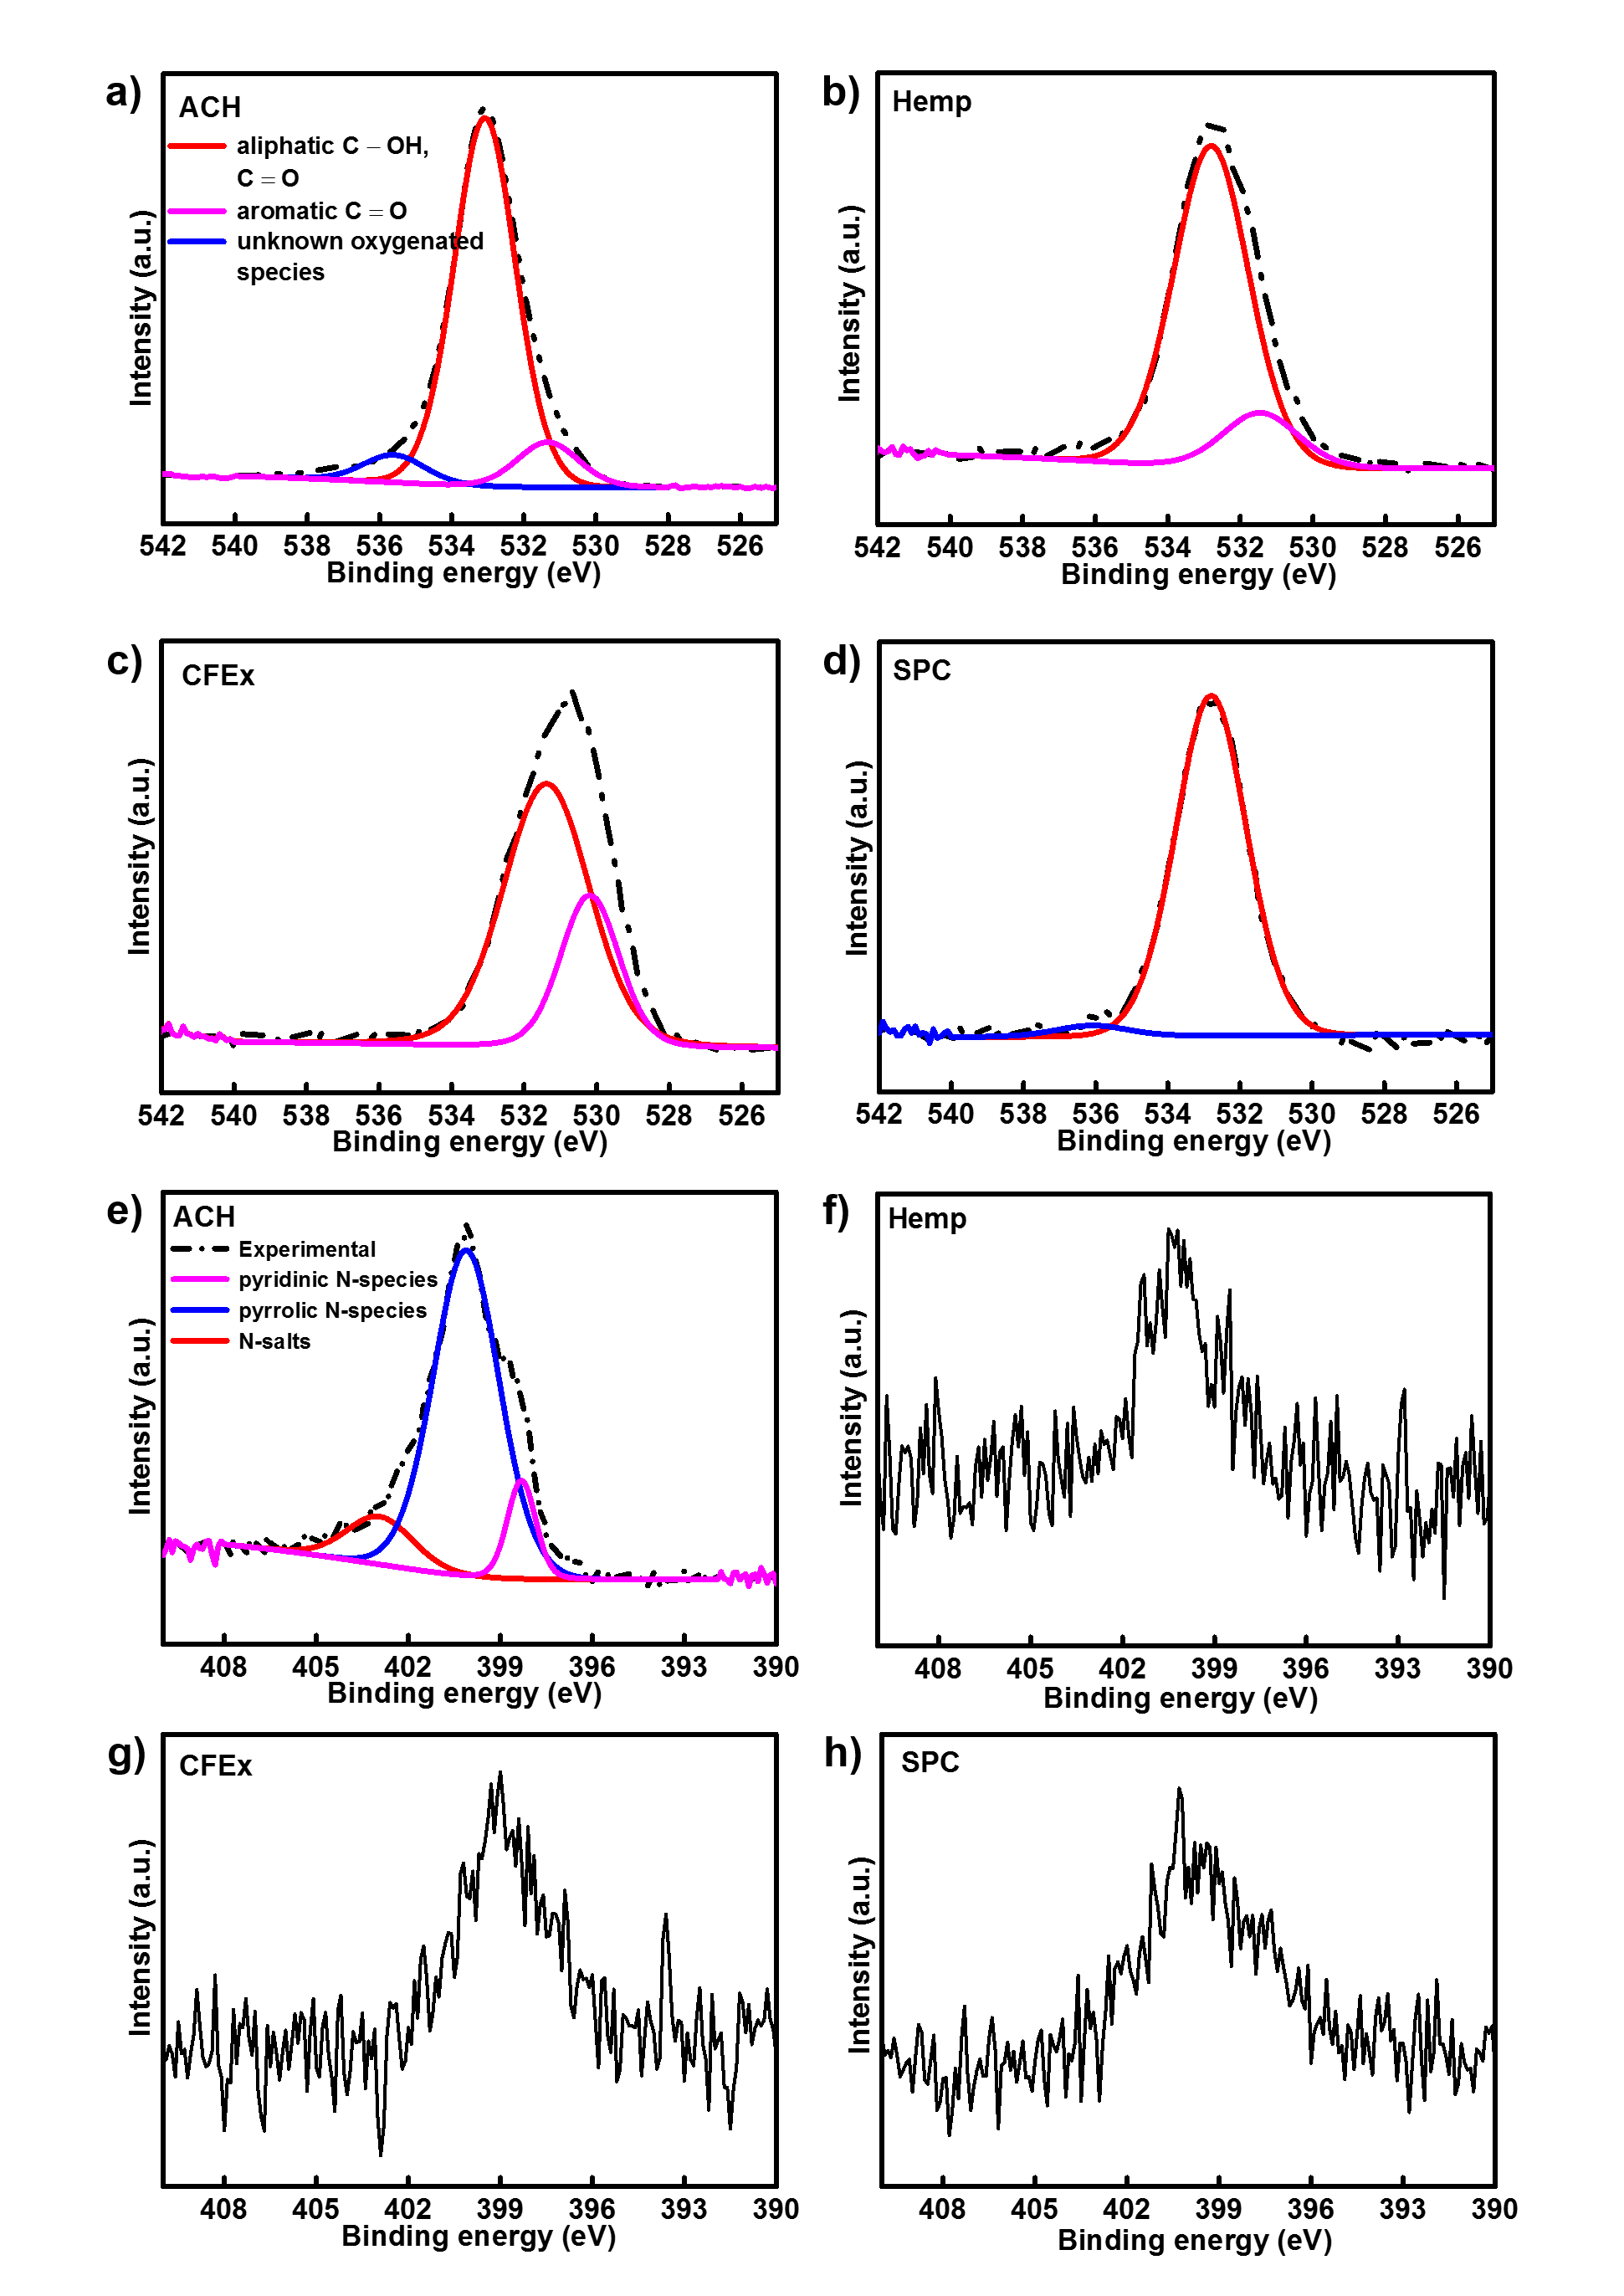
\includegraphics[width=0.8\textwidth]{figures/XPSON}
    \caption{XPS spectra of O 1s orbital for a) human hair, b) hemp fibers c) CFEx and d) SPCB cathodes. Hair and hemp fibers contained significant amounts of aliphatic (red) and aromatic (pink) C=O groups  compared to CFEx and SPCB. Binding energies for N 1s orbital of e) hair, f) hemp fibers g) CFEx and h) SPCB cathodes. Human hair displayed distinct binding energies for pyridinic and pyrrolic N-species; hemp fibers, CFEx and SPCB had smaller amounts of surface proteins.}
  \label{figures:XPSON}
\end{figure}

Figure \ref{figures:XPSON}a-d shows various binding energies for O 1s orbital. As mentioned earlier, oxygen-containing functional groups enhance the wettability of a material and presence of oxygen atoms make redox reactions feasible \cite{li_effect_2011, oh_oxygen}. Oxygen-containing surface functional groups can provide pseudo-capacitance by reacting with electrolyte ions \cite{bleda_martinez}. This might be one of the reasons why aluminium-hair and aluminium-fullerene batteries performed better than others. 

 \begin{figure}[tbh!]
  \centering
  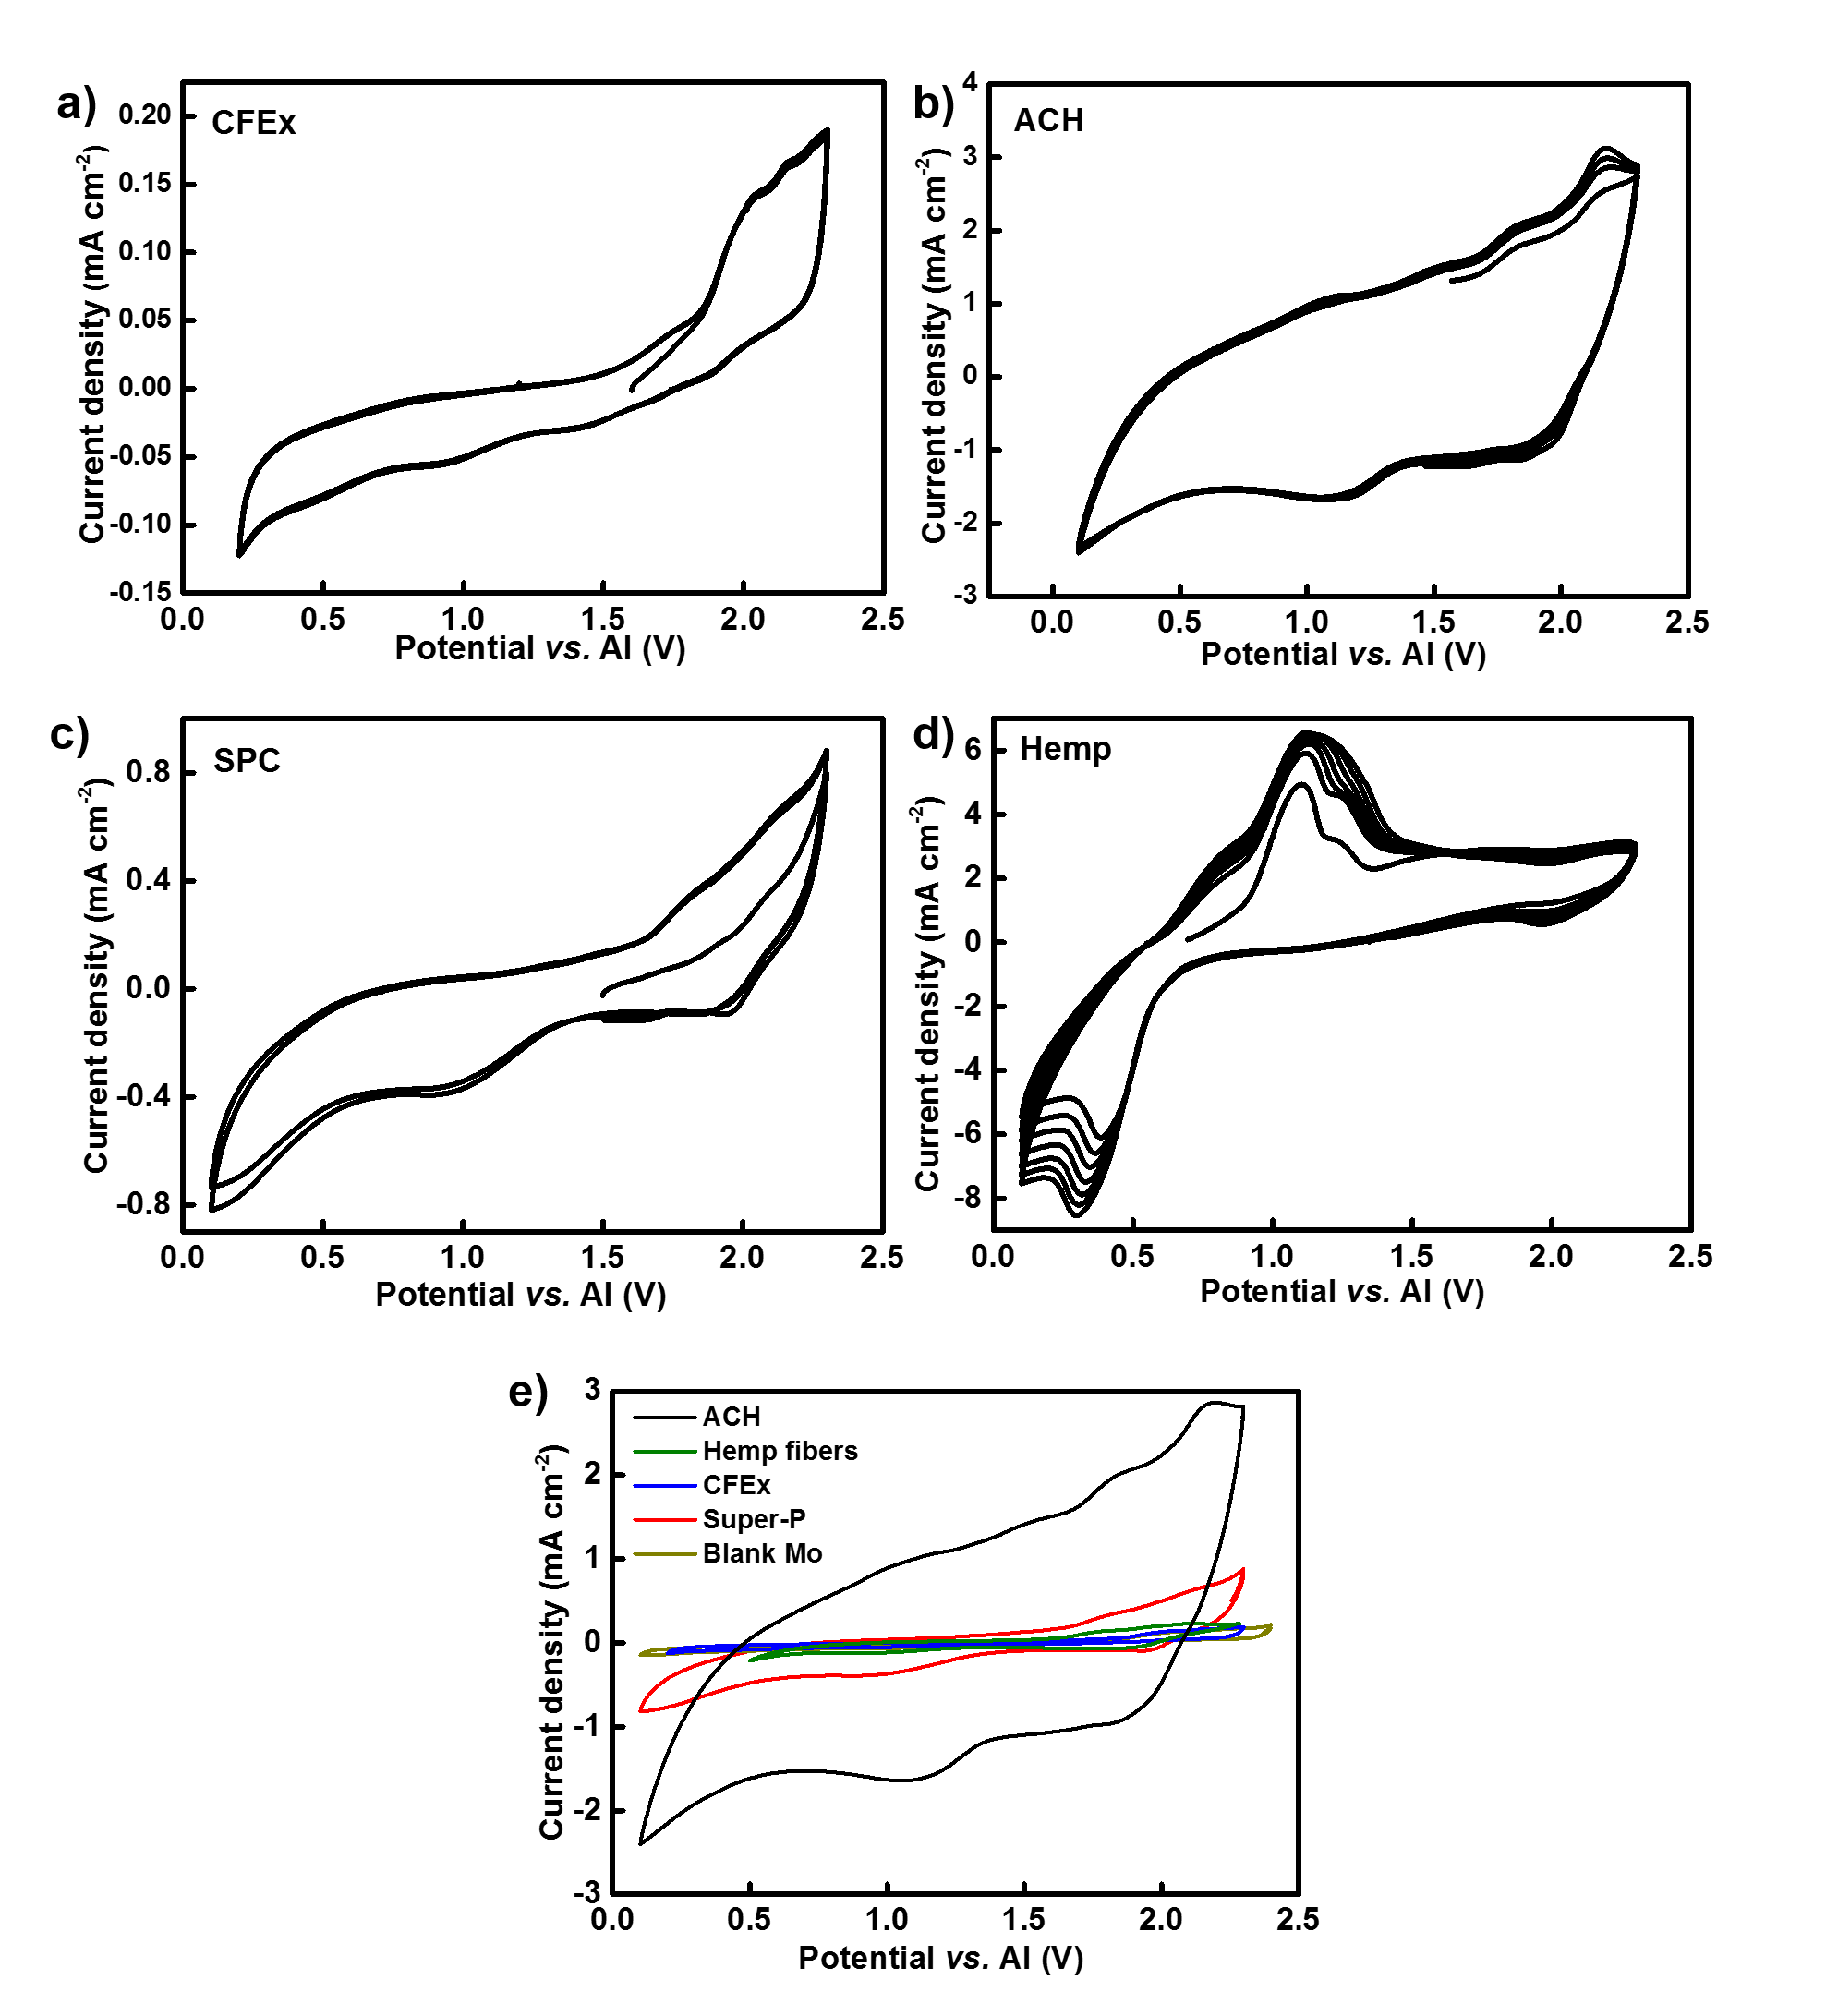
\includegraphics[width=\textwidth]{figures/CV}
    \caption{Cyclic voltammograms of a) CFEx, b) ACH, c) Super-P and d) hemp fibers cathodes at a scan rate of 10 mV s$^{-1}$ against \ce{Al3+}/Al as a counter/reference electrode in a two-electrode setup. ACH cathode observed a larger CV area than other cathodes, which comes from an additional pseudocapacitance, adding capacity to the system.}
  \label{figures:CV}
\end{figure}

Lastly, to confirm that ACH is a psedocapacitive material, we compared cyclic voltammograms of all cathodes at a scan rate of 10 mV s$^{-1}$. From Figure \ref{figures:CV}a-e, it was seen that human hair had a rectangular capacitor-like CV curve. However, redox processes were noticeable at a lower scan rate (10 mV s$^{-1}$) and tiny redox peaks visible (Figure \ref{figures:CV}b). At a higher scan rate (50 mV s$^{-1}$), the redox peaks disappeared and the material displays solely a capacitor-like behaviour, shown in Figure \ref{SF:hair50mVs} \cite{guan_capacitive, dupont_separating}. 

 \begin{figure}[tbh!]
  \centering
  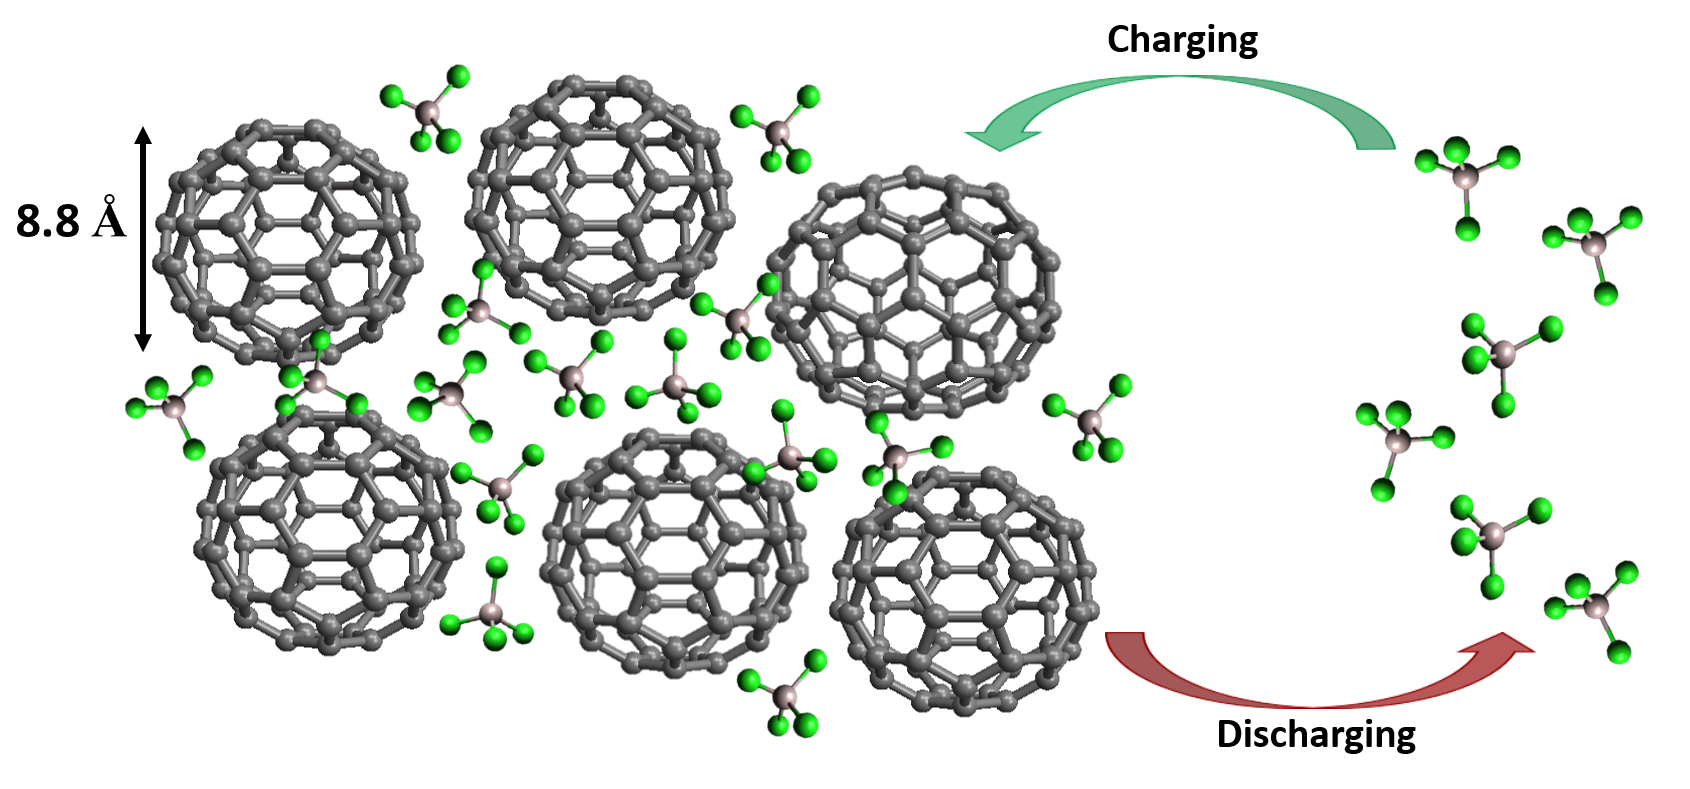
\includegraphics[width=\textwidth]{figures/CFExmech}
    \caption{Suggested mechanism for a \textbf{Al/CFEx} cell. \ce{AlCl4-} ions seeping in through the gaps present between fullerene molecules. A few \ce{AlCl4-} ions get absorbed on the cathode's surface resulting in a capacity purely from a non-Faradaic process.}
  \label{figures:CFExmech}
\end{figure}

\begin{figure}[tbh!]
  \centering
  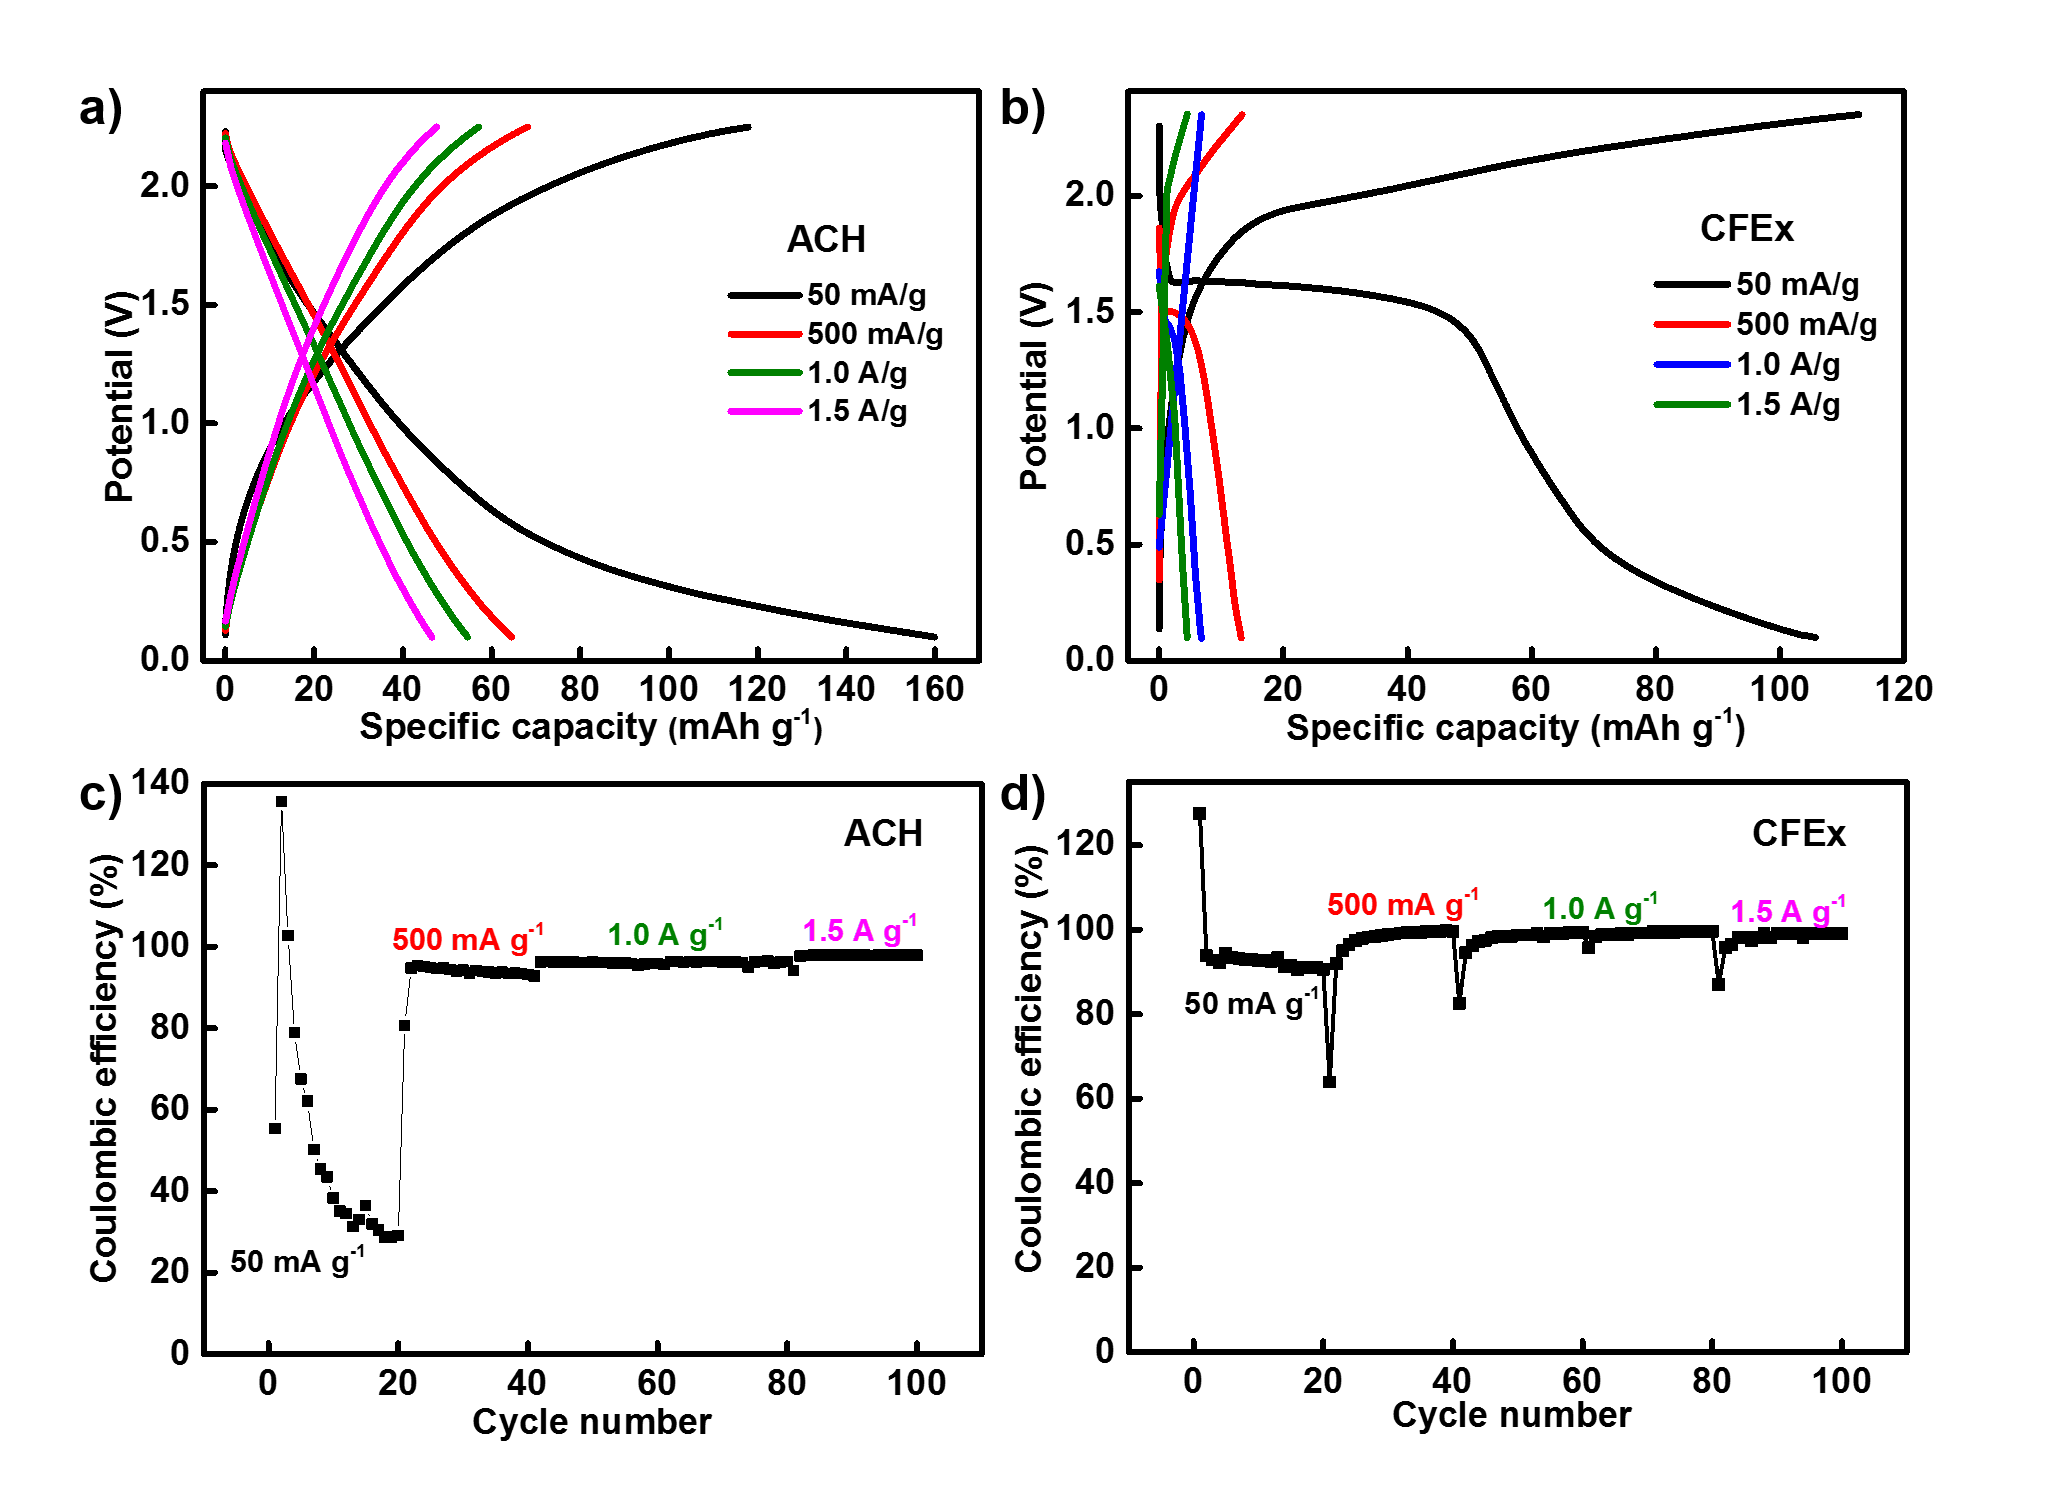
\includegraphics[width=\textwidth]{figures/CFExACHlong}
    \caption{Discharge capacities of a) ACH and b) CFEx cathodes at current rates of 50mAg$^{-1}$, 500mAg$^{-1}$, 1.0 Ag$^{-1}$ and 1.5 Ag$^{-1}$ along with their coulombic efficiencies. }
  \label{figures:CFExACHlong}
\end{figure}

% Are the following the conclusions?
\section{Conclusion}
ACH proved to be the best carbon-based cathode among all the tested materials, with a specific capacity of 100 mAh g$^{-1}$ at a potential of 1.9 V with a coulombic efficiency of $\sim$90$\%$. Intercalation and deintercalation of \ce{AlCl4-} takes place in the very few graphitic layers of ACH, hemp fibers and Super-P. We found that CFEx lacks a layered structure and it is mainly a cluster of \ce{C60} and \ce{C70} molecules. \ce{AlCl4-} anions seep in and out of the gaps in between the fullerenes changing its structure during insertion and expanding the crystal lattice (Figure \ref{figures:CFExmech}). Since the cathode maintains its structural integrity, the coulombic efficiency remains stable throughout the cycles for CFEx cell. Hemp fibers and Super-P on the other hand, have a highly amorphous structure and degrades after every cycle, resulting in a low capacity value. Figure \ref{figures:CFExACHlong} compares the 50th cycle measurement for Al/ACH and Al/natural graphite cell. It not only displays a higher specific capacity than conventional graphite, but also a high battery voltage of 1.92 V with an energy density of 202 Wh kg$^{-1}$.

\section{Experimental Section}
\subsection{Chemicals}
\subsubsection*{Activated carbon from human hair}
\subsubsection*{Activated carbon from hemp fibers}
The material was provided by Carbon Valley and used as received.
\subsubsection*{Fullerene extract}
C60/C70, approx. 85\% C60, 14\% C70, and 1\% higher fullerenes, was purchased from SES research and used as received.
\subsubsection*{Super-P carbon black}
Super-P conductive carbon, 99+\% metals basis was purchased from Alfa-Aesar and used as received


\subsection{Cathode preparation}
A slurry was prepared by mixing the active material (85$\%$ by wt.), 9$\%$ binder (PVDF, MTI Corp.) and 6$\%$ Super-P conductive carbon (99+$\%$ metals basis, Alfa Aesar) in N-methyl pyrrolidone NMP (anhydrous, 99.5$\%$, Sigma-Aldrich). For SPCB slurry 94$\%$ active material and 6$\%$ binder was mixed together to form a slurry. It was ‘doctor-bladed’ on molybdenum foil used as a conductive substrate (thickness 0.1 mm, MTI Corp.) and dried in a vacuum oven at 120$^{\circ}$C for 12 hours to adhere the slurry on the substrate and evaporate the solvent. Specific loading of the materials ranged from 11-12 mg cm$^{-2}$. 

\subsection{Electrolyte preparation}
Anhydrous \ce{AlCl3} (Sigma-Aldrich) and EMImCl (97$\%$, Sigma-Aldrich) were mixed in a molar ratio of 1.3:1, at room temperature. EMImCl was baked in vacuum for 24 hours at 100$^{\circ}$C to remove residual moisture. Small aliquots of AlCl$_3$ was added to EMImCl after every few minutes. The ionic liquid was stirred for 2-3 hours until a clear brown liquid was obtained. Since the electrolyte is hygroscopic in nature, it was prepared in a N$_2$-filled glove box with <0.1 ppm H$_2$O/O$_2$. 

\subsection{Cell assembly}
PEEK (polyether ether ketone) cells were used for electrochemical measurements (Figure \ref{SF:PEEK}). Molybdenum rods were used as current collectors. It was seen previously that steel rods reacted with the electrolyte forming a green-colored substance on the cathode. The slurry coated on molybdenum foil was used as the cathode and placed at bottom of the cell. Two glass microfibers (Grade GF/F, Whatman) were used as separators. 80$\mu$l of the electrolyte was used to wet the separator. Aluminium foil (thickness 0.1 mm, 99$\%$, GoodFellow) used as an anode and placed on top of the separator. It was assembled in a N$_2$-filled glove box. The cell was then sealed and wrapped with a paraffin film to avoid any air or moisture contact. Since this was a two-electrode setup, aluminium foil was used as both counter and reference electrode. The cell was taken out of the glove box and electrochemical measurements were performed. 

% What is this figure doing here in the wild?
%\begin{figure}[tbh!]
 % \centering
  %
\includegraphics[width=\textwidth]{figures/GCDCall}
   % \caption{Chronopotentiographs (Voltage vs. Time) curves of all tested cathodes.}
  %\label{figures:GCDCall}
%\end{figure}

\section{Conclusions}

% Where are the conclusions?


%\documentclass{article}
\usepackage{arxiv}
\usepackage[utf8]{inputenc} % allow utf-8 input
\usepackage[T1]{fontenc}    % use 8-bit T1 fonts
\usepackage{hyperref}       % hyperlinks
\usepackage{url}            % simple URL typesetting
\usepackage{booktabs}       % professional-quality tables
\usepackage{amsfonts}       % blackboard math symbols
\usepackage{nicefrac}       % compact symbols for 1/2, etc.
\usepackage{microtype}      % microtypography
\usepackage{lipsum}
\usepackage{upgreek}
\usepackage{graphicx}
\usepackage[version=4]{mhchem}
\usepackage{gensymb}
\usepackage{verbatim}
\usepackage{amsmath}
\usepackage{amssymb}

\title{Carbon cathodes for rechargeable aluminium-ion batteries}
\author{
Shalini Divya\\
  School of Chemical and Physial Sciences\\
  Victoria University of Wellington\\
  Wellington, New Zealand\\
  \texttt{shalini.divya@vuw.ac.nz}\\
  %% examples of more authors
   \And
  Thomas Nann\thanks{Corresponding author.}\\
  School of Mathematical and Chemical Sciences\\
  The University of Newcastle\\
  Newcastle, NSW 2308, Australia\\
  \texttt{thomas.nann@newcastle.edu.au}\\
}


\begin{document}
\maketitle
\section*{Supporting Information}
\newcommand{\beginsupplement}{
               \setcounter{figure}{0}
        \renewcommand{\thefigure}{S\arabic{figure}}
     }
\beginsupplement


\begin{figure}[ht!]
\centering
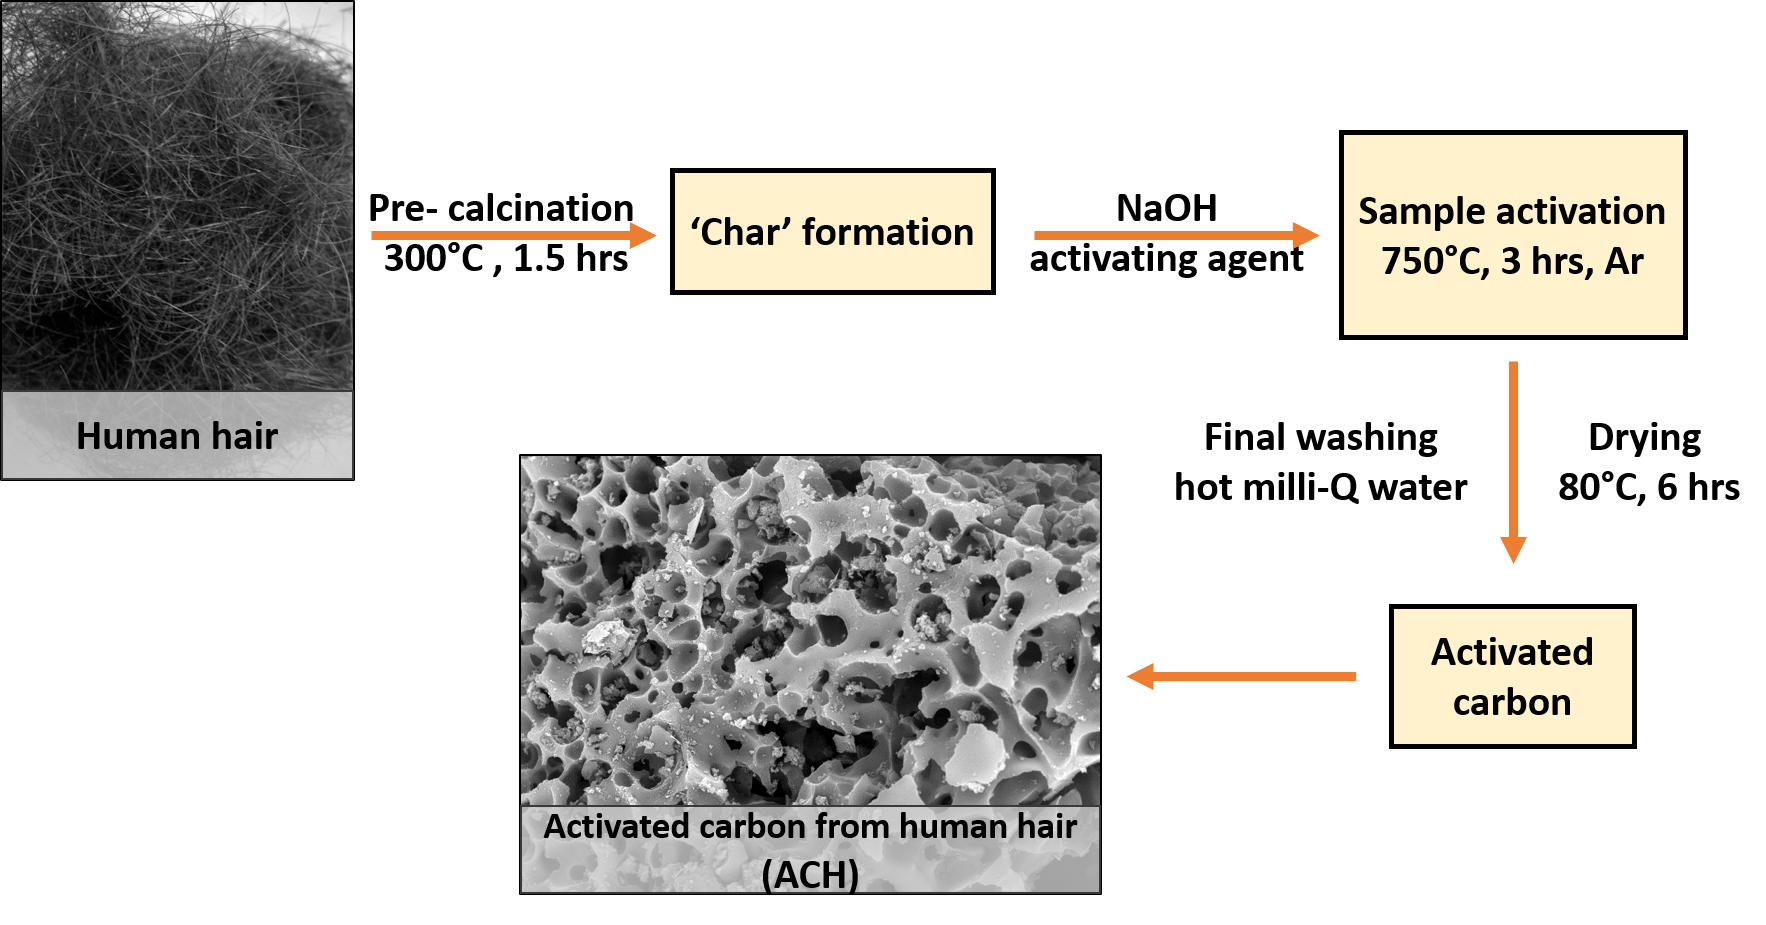
\includegraphics[width=\textwidth]{fig/ACHsyn}
\caption{Synthesis of activated carbon from human hair using NaOH as the activating agent.}
\label{fig:ACHsyn}
\end{figure}

\begin{figure}[th!]
\centering
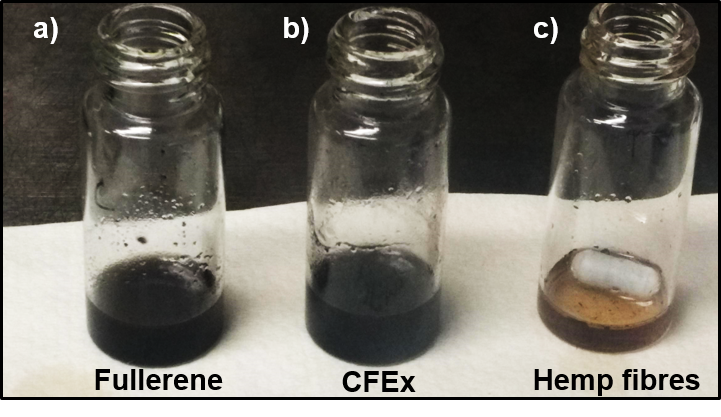
\includegraphics[width=\textwidth]{fig/CFExsol}
\caption{Synthesis of activated carbon from human hair using NaOH as the activating agent. The choice of temperature and activating agent plays a crucial role in determining pore size of the activated carbon.}
\label{fig:CFExsol}
\end{figure}

\begin{figure}[th!]
\centering
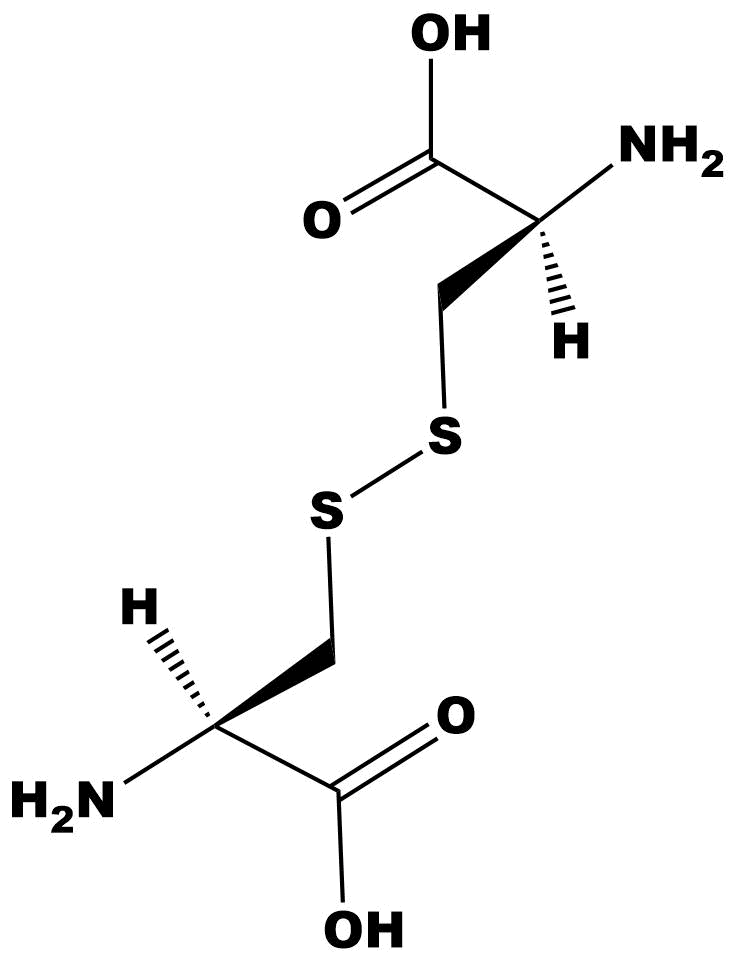
\includegraphics[width=0.5\textwidth]{fig/keratin}
\caption{Keratin: a protein abundantly found in human hair contains C-O, C=O, C-NH$_2$ bonds.}
\label{fig:keratin}
\end{figure}

\begin{figure}[th!]
\centering
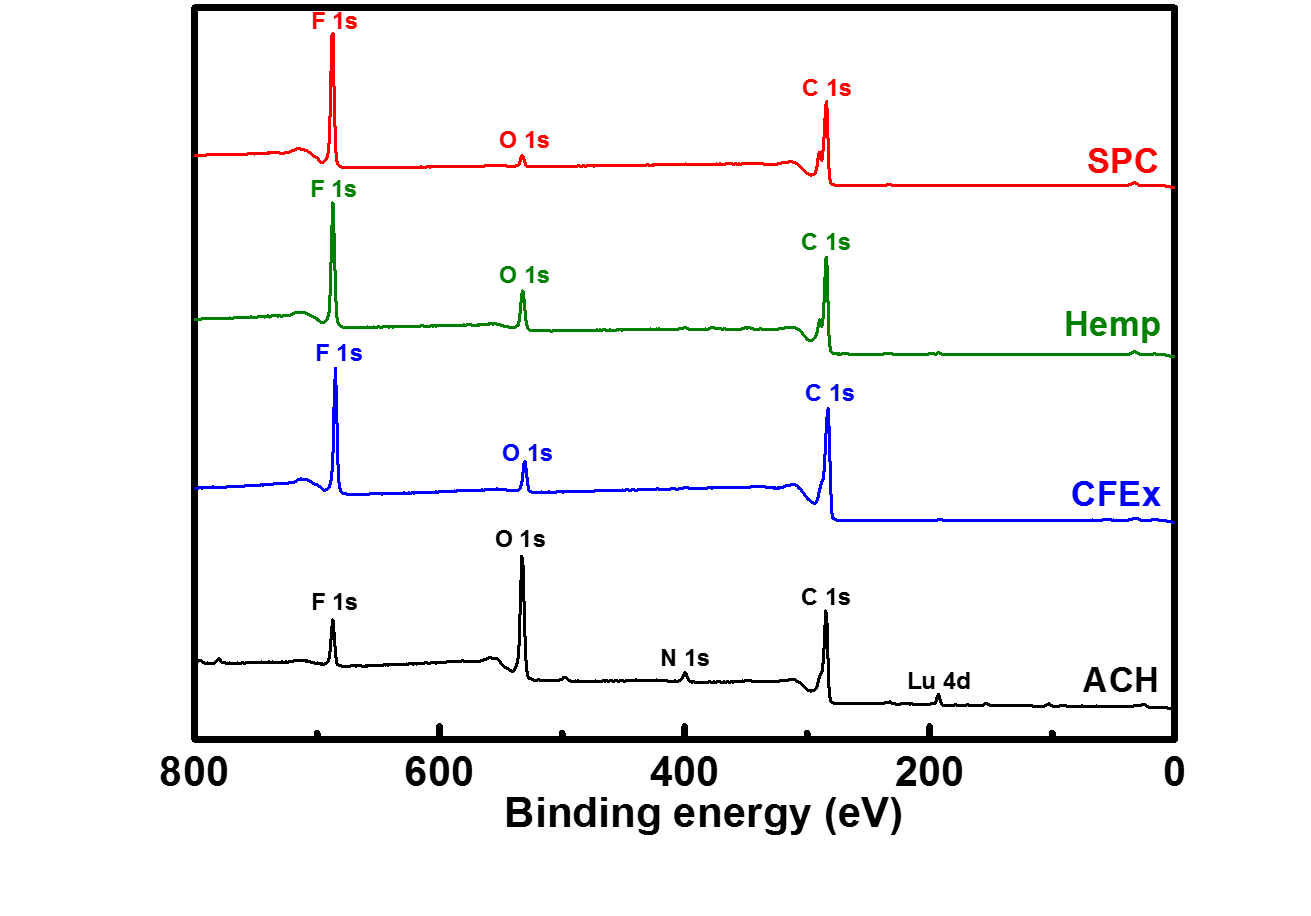
\includegraphics[width=\textwidth]{fig/XPSoverall}
\caption{Overall spectra of ACH (blck), hemp fibers (blue), CFEx (green) and SUper-P(red).}
\label{fig:XPSoverall}
\end{figure}

\begin{figure}[th!]
\centering

\includegraphics[width=\textwidth]{fig/hair50mVs}
\caption{Cyclic voltammogram of ACH at a scan rate of 50 mV/s in a two electrode setup against \ce{Al3+}/Al showing a capacitor-like behaviour with no visible oxidation-reduction peaks unlike Figure \ref{fig:CV}b where we distinctly observed redox peaks.}
\label{fig:hair50mVs}
\end{figure}

\begin{figure}[th!]
\centering
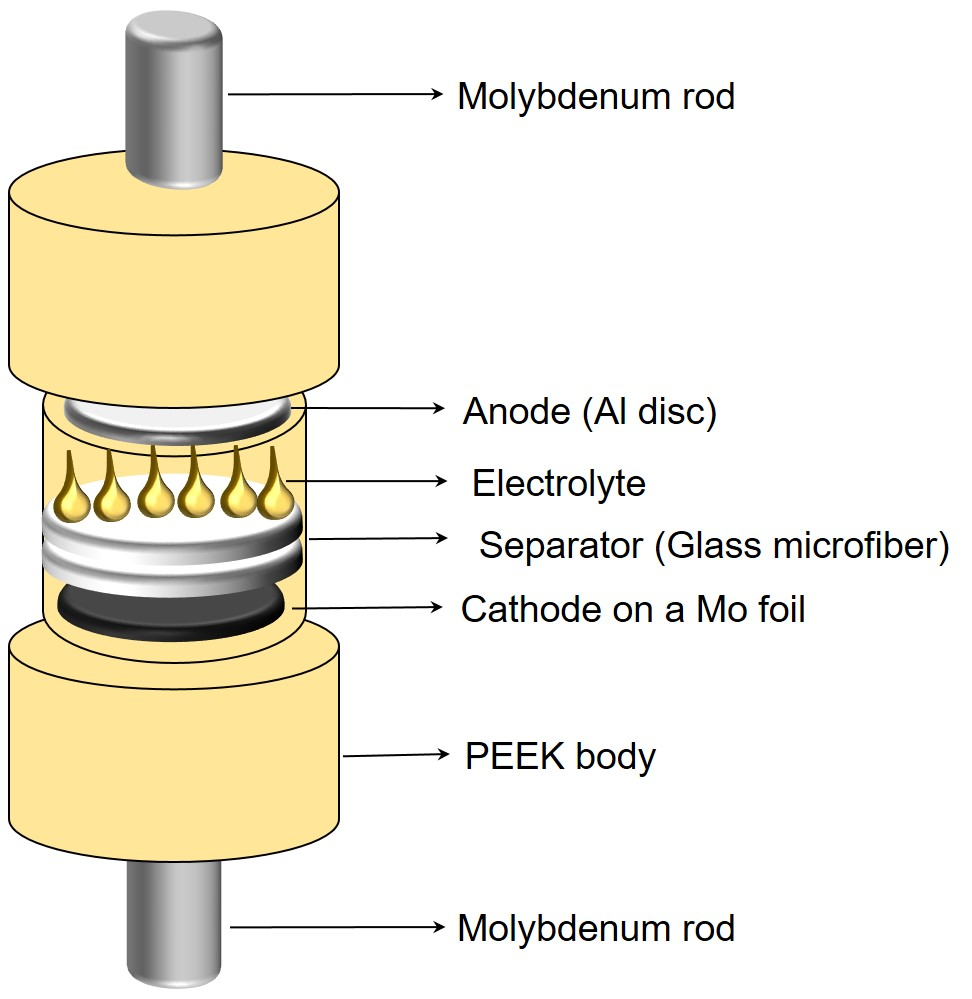
\includegraphics[width=\textwidth]{fig/PEEK}
\caption{A custom-made two-electrode polyetherether ketone (PEEK) cell used for galvanostatic cycles and cyclic voltammetry.}
\label{fig:PEEK}
\end{figure}

\end{document} % This should be a separate file.

\bibliographystyle{unsrt}  % Something must be wrong here....
\bibliography{thesis} 


\end{document}
